\documentclass[sigconf]{acmart} % authordraft

\usepackage{booktabs} % For formal tables

\usepackage{hyperref}
\usepackage{amsmath,amssymb,mathtools}
\usepackage{xr}
% \usepackage{float}
% \usepackage{stackengine}


% Copyright
\copyrightyear{2018} 
\acmYear{2018} 
\setcopyright{acmcopyright}
\acmConference[GECCO '18]{Genetic and Evolutionary Computation Conference}{July 15--19, 2018}{Kyoto, Japan}
\acmBooktitle{GECCO '18: Genetic and Evolutionary Computation Conference, July 15--19, 2018, Kyoto, Japan}
\acmPrice{15.00}
\acmDOI{10.1145/3205455.3205529}
\acmISBN{978-1-4503-5618-3/18/07}


\begin{document}

\title{Interoceptive robustness through environment-mediated morphological development}

\author{Sam Kriegman}
\affiliation{%
  \institution{University of Vermont}
  \city{Burlington} 
  \state{VT} 
  \country{USA}
}
\email{sam.kriegman@uvm.edu}

\author{Nick Cheney}
\affiliation{%
  \institution{University of Wyoming}
  \city{Laramie} 
  \state{WY} 
  \country{USA}
}

\author{Francesco Corucci}
\affiliation{%
  \institution{3DNextech s.r.l.}
  \city{Livorno} 
  \country{Italy}
}

\author{Josh C. Bongard}
\affiliation{%
  \institution{University of Vermont}
  \city{Burlington} 
  \state{VT} 
  \country{USA}
}



% The default list of authors is too long for headers.
\renewcommand{\shortauthors}{Kriegman et al.}


\begin{teaserfigure}
\centering
\vspace{-1.75em}
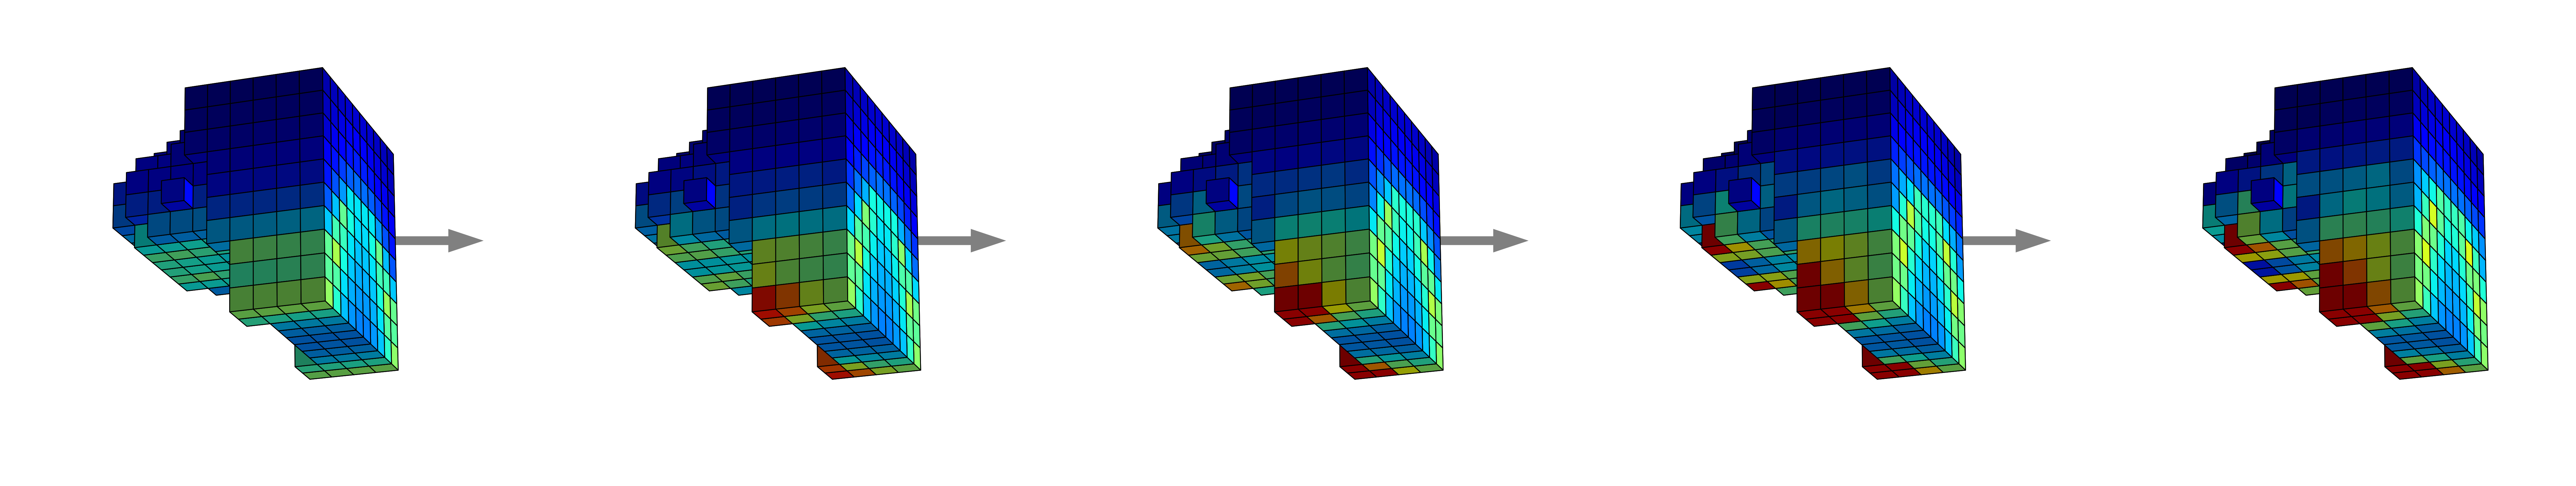
\includegraphics[width=\linewidth]{img/Callosities} \\
\vspace{-1.75em}
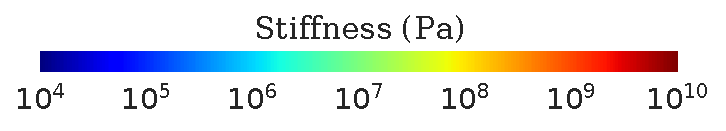
\includegraphics[width=0.35\linewidth]{img/colorbar} \\
\vspace{-1em}
\caption{A single robot grows calluses as it walks, 
% rigidifying
in response to pressure on its feet   
(\href{https://youtu.be/0cmwpcxSUWI}{\textcolor{blue}{\textbf{\texttt{youtu.be/0cmwpcxSUWI}}}}).
} % (The champion of run 6.)
\label{fig:calluses}
\vspace{1em}
\end{teaserfigure}


\begin{abstract}
% Abstract length should not exceed 200 words

Typically, AI researchers and roboticists try to realize
intelligent behavior in machines by tuning parameters of a 
predefined structure (body plan and/or neural network
architecture) using evolutionary or learning algorithms. 
Another but not unrelated longstanding property of these systems is their brittleness to slight aberrations, as highlighted by the growing deep learning literature on adversarial examples.
Here we show robustness can be achieved by
evolving the 
geometry of soft robots, their
control systems, and how
their material properties develop
in response to one particular interoceptive stimulus
(engineering stress) during their lifetimes.
By doing so we realized robots that 
were equally fit but more robust to 
extreme material defects (such as 
might occur during fabrication or by damage thereafter)
than robots that did not develop during their lifetimes,
or developed in response to a different interoceptive
stimulus (pressure).
This suggests that the interplay between changes
in the containing systems
of agents (body plan and/or neural architecture)
at different temporal scales (evolutionary
and developmental) along different modalities
(geometry, material properties, synaptic weights)
and in response to different signals (interoceptive
and external perception) all
dictate those agents' abilities to evolve or 
learn capable and robust strategies.
\end{abstract}


%
% The code below should be generated by the tool at
% http://dl.acm.org/ccs.cfm
%
\begin{CCSXML}
<ccs2012>
<concept>
<concept_id>10010147.10010178.10010219.10010222</concept_id>
<concept_desc>Computing methodologies~Mobile agents</concept_desc>
<concept_significance>500</concept_significance>
</concept>
</ccs2012>
\end{CCSXML}

\ccsdesc[500]{Computing methodologies~Mobile agents}


\keywords{Soft robotics.}





\maketitle

\section{Introduction}
\label{sec6:introduction}

A major characteristic of life is that three broad time scales are relevant to it: evolution, development and physiological functioning.
% \citep{waddington1957strategy}.
Engineered systems, in marked contrast, often employ an evolutionary or learning algorithm to improve their behavior over time, but rarely employ morphological development; any changes to the physical layout are made in between evaluations \citep{sims1994evolving,lipson2000automatic,cheney2013unshackling}, if they are made at all.

Two notable exceptions are modular robots \citep{zykov2005robotics}, which may reconfigure their bodies by adding and removing discrete structures, and soft robots \citep{shepherd2011multigait}, which may continuously alter the local volumes of different parts of their
bodies while behaving. 
Others \citep{bongard2011morphological} have approximated topological change in rigid bodies by extending outward and angling downward 
appendages using a combination of linear and rotary actuators, thus simulating limb growth.

Several computational but embodied models of \textit{prenatal} development have been reported in the literature \cite{dellaert1996developmental,
% dellaert1994toward,
Eggenberger97,
Bongard01,
% bongard2003evolving,
miller2004evolving,
doursat2009organically}.
As implied,
cellular growth therein occurred prior to any physiological functioning. 
Thus, these studies included change during only
two of the three time scales relevant to life:
evolutionary and behavioral change, but not postnatal developmental
change.

The most common argument in favor of development is that some aspects of the environment are unpredictable, so it is advantageous to leave some decisions up to development rather than specifying them genetically.
Although self evident, it remains to determine which mechanisms of development should be instantiated in robots to realize plastic, adaptive, and useful machines.

Naturally, the performance of an evolved system depends on its capacity for evolutionary improvement: its evolvability.
Development can, under certain conditions, smooth the search space evolution that operates in, thus increasing evolvability.
This process, known as the Baldwin effect \citep{baldwin1896new,dennett2003baldwin}, starts with an advantageous characteristic acquired during the development of individuals, such as the callouses in Fig. \ref{fig6:calluses}. 
This can create a new gradient in the evolutionary search space, rewarding descendants that more rapidly manifest the trait during their lifetimes \citep{hinton1987learning,kriegman2018morphological}
and retain it through the remainder of their lifetime \citep{kriegman2017minimal}.
Assuming such mutations exist and can be naturally selected \citep{kriegman2018morphological}, following the gradient requires incrementally reducing development in the manifold of the search space that can express variations on the trait \cite{waddington1942canalization}.


However, fitness landscapes that evolution climbs, and development sometimes smooths, tend not to remain static in realistic settings.
On this vacillating landscape, when the best thing to do does not remain the same, a highly evolvable but non-robust system will need to keep starting over from scratch every time the conditions change.
Computational and engineered systems provide countless examples of systems with nearly perfect performance in a controlled environment, such as a factory, but who turn out to be (often comically) brittle to slight changes in their internal structure, such as damage, or their external environment such as moving on to new terrain or transferal from simulation to reality 
\citep{carlson2005ugvs,
koos2013transferability,
% mccloskey1989catastrophic,
% french1999catastrophic,
goodfellow2013empirical,
szegedy2013intriguing,
% goodfellow2014generative,
athalye2018synthesizing,
% gilmer2018adversarial,
% su2017one,
nguyen2015deep}.

Although generally absent from engineered systems (but see \cite{bongard2006resilient,cully2015robots}), the canonical form of robustness is seen to some extent in all organisms, and it comes from the act of development itself.
For example, a plant that grows according to a fixed program will capture less light than a plant that grows toward sunlight.
But there is another, more subtle form of robustness that we will refer to as `intrinsic robustness' because it is a property of a system's structure rather than of the process by which it may change.

Developmental change produces intrinsically robust systems because they evolved from designs that had to maintain adequate performance along additional dimensions of change \citep{bongard2011morphological,kriegman2018morphological}.
Through morphological development specifically, evolution is compelled to maintain designs that are capable across a series of body plans, with different 
% behavioral repercussions of action, and different 
sensor-motor contingencies; and the ability to tolerate such perturbations can become inherited to some extent in descendants' behaviors \cite{bongard2011morphological} and morphologies \cite{kriegman2018morphological}, even when their developmental flexibility is reduced or completely removed by canalization or fabrication.


And yet, despite the ubiquity of
% (postnatal) 
morphological development in nature, and the adaptive advantages it seemingly confers, there are only a handful of cases reported in the literature in which a simulated robot's mechanical structure was allowed to change while it was behaving 
(e.g.~\citep{ventrella1998designing,
komosinski2003framsticks,
bongard2011morphological,
kriegman2018morphological,
kriegman2017minimal}),
all of which modeled morphological development as a genetically predetermined process: the environment could not influence the way in which development unfolded. 


Assuming that an engineered system is capable of local morphological change in response to environmental signals, it is unclear how it should do so, beyond the examples of morphological plasticity observed in nature. 
Examples include Wolff's law \citep{ruff2006s}---bone grows in response to particular mechanical loading profiles---and Davis' law---soft tissue increases in strength in response to intermittent mechanical demands.
One can envisage other such laws that are not known to occur in biology but could be helpful in a specific artificial system, such as end effectors softening in response to pressure, which might enhance their ability to safely manipulate irregular or delicate objects \cite{brown2010universal}.
Indeed, the genesis of the work presented here is one such anecdotal example given in \citep{corucci2017evolutionary}, where a single robot, subjected to an abrupt doubling in gravity, stiffened its body in reaction to the increased pressure.
However, whether or how it could provide a behavioral advantage, nor whether pressure is the best interoceptive signal to developmentally respond to,
was not investigated.

As a step towards a more adequate picture, we introduce here a simple form of a developmental feedback mechanism:
Genetic systems dictate how organisms develop in response to interoceptive stimuli, and development alters the kinds of interoceptive conditions the organism experiences.
More specifically, at every time step, the proposed model of closed-loop development:
\begin{enumerate}
\item `listens to' load signatures generated from movement; and, in response,
\item modifies the robot's rigidity,
\end{enumerate}
which will change the way it distributes load and generates movement at the next time step.


Optimizing a system that may form a continuum of rigid and soft components---and in which this admixture may change over time---is extremely nonintuitive and underexplored.
Thus, a study of the adaptive properties of such systems---and how they can best be optimized to render useful work---is initiated here.



\section{Methods}
\label{sec:methods}

We evolved locomotive machines constructed from voxels with heterogeneous stiffness. 
Like many organisms \citep{ruff2006s}, the robot's material stiffness progressively changes in response to mechanical loading incurred as the robot behaves.
This ontogenetic change occurs independently at each voxel according to an evolved local rule.


\subsection{Physical simulation.}

The soft-matter physics engine \textit{Voxelyze} \citep{hiller2014dynamic} is used to calculate the movement of robots resulting from their interaction with a virtual 3D terrestrial environment.
Each robot is simulated for 25 times the length of an expansion/contraction cycle (a total of five seconds). 
The displacement between the starting coordinates and the agent's final center of mass (in the $xy$ plane) is recorded.\footnote{\href{https://github.com/skriegman/2018-gecco}{\textcolor{blue}{\textbf{\texttt{github.com/skriegman/2018-gecco}}}} contains the source code necessary for reproducing the results reported in this paper.}


% For a more general purpose repository see \href{https://github.com/skriegman/evosoro}{\textcolor{blue}{\textbf{\texttt{github.com/skriegman/evosoro}}}}


\subsection{Heavy materials.}

% 1e6 -> 1e9 density
% vol = length^3
% mass = vol * density 
% previously each voxel was a centimeter in length and one gram in mass.
% now each voxel is 1 kg/cm^3 in mass, which is heavier than the heaviest material on earth (22 g/cm^3) so this calculation is incorrect. 

Materials are simulated to have increased mass relative to those used by \cite{hiller2012automatic,cheney2013unshackling,cheney2014electro}.
Constructed from heavier materials, many previously mobile robots become crushed under their own weight and require stiffer material to support locomotion with the same geometry.
However, we also restricted actuation amplitude as materials grow stiffer to better approximate the properties of real materials with different stiffnesses.
This creates an interesting and realistic trade-off: the stiffest material can easily support any body plan but cannot move on its own (like a skeleton without muscle), whereas the softest material can readily elicit forward movement in smaller bodies but cannot support many larger and potentially faster-moving body plans, 
such as those with narrow supporting limbs.
Thus, a robot must carefully balance support with actuation.



\subsection{Quad-CPPN encoding: $\mathbf{\mathbb{C}_1,\mathbb{C}_2,\mathbb{C}_3,\mathbb{C}_4}$
}

Following \cite{cheney2013unshackling}, robot physiology is genetically encoded by a Compositional Pattern Producing Network (CPPN) \citep{stanley2007cppn}, a scale-free mapping that biases search toward symmetrical and regular patterns which are known to facilitate locomotion.


Each point on a 10$\times$10$\times$10 lattice is queried by its cartesian coordinates in 3D space and its radial distance from the lattice center.
An evolved CPPN takes these coordinates as input and returns a single value which is used to set some property of that point in the workspace.
We used four independent CPPNs to separately encode: Geometry, Stiffness, Development, and Actuation.



\subsection{$\mathbf{\mathbb{C}_1}\;$ Geometry.}
The geometry of a robot is specified by a bitstring that indicates whether material is present (1) or absent (0) at each lattice point in the workspace, as dictated by $\mathbb{C}_1$.
The robot's geometric shape is taken to be the largest contiguous collection of present voxels.


\subsection{$\mathbf{\mathbb{C}_2}\;$ Stiffness.}
Young's modulus is often used as an approximate measure of material stiffness.
Robots are typically constructed of materials such as metals and hard plastics that have moduli in the order of $10^9 - 10^{12}$ pascals (Pa), whereas soft robots (and natural organisms) are often composed of materials with moduli in the order of
$10^4 - 10^9$ Pa \citep{rus2015design}.


Here, voxels may have moduli in the range $10^4 - 10^{10}$ Pa.
The robot's congenital stiffness is set at each voxel by $\mathbb{C}_2$, but may be changed by development.



% ``Young's modulus is only defined for homogeneous, prismatic bars that are subject to axial loading and small deformations ($< 0.2\%$ elongation for metals) and thus has limited relevance to soft robots and other soft-matter technologies that have irregular (non-prismatic) shape and undergo large elastic or inelastic deformations. Nonetheless, Young’s modulus is a useful measure for comparing the rigidity of the materials that go into a soft robot.'' - Majidi \citep{majidi2014soft}


\subsection{$\mathbf{\mathbb{C}_3}\;$ Development.}
The robot's stiffness distribution $k$ 
can change progressively during its lifetime $t$ in response to localized engineering stress $\sigma$ or pressure $p$.
The rate of change $\alpha_i$ is specified at the $i^{\text{th}}$ voxel by $\mathbb{C}_3$, with possible values in $0\pm10$.
We compare three developmental variants.
% We compare the following developmental variants.
\begin{align}
% \shortintertext{\textit{\textbf{None:}}} 
&\textit{\textbf{None:}} 
\hspace{2em} &\frac{dk_i}{dt}& \,=\, 0 
\hspace{10em}
\label{eq:none} \\[0.35em]
% \shortintertext{\textit{\textbf{Stress:}}}
&\textit{\textbf{Stress:}} \hspace{3em} &\frac{dk_i}{dt}& \,=\, \alpha_i \cdot \frac{d\sigma_i}{dt} 
\label{eq:stress} \\[0.35em]
% \shortintertext{\textit{\textbf{Pressure:}}}
&\textit{\textbf{Pressure:}} \hspace{3em} &\frac{dk_i}{dt}& \,=\, \alpha_i \cdot \frac{dp_i}{dt} 
\label{eq:pressure}
\end{align}
% \\[1em]
% \intertext{As an additional control, we include ballistic development \citep{kriegman2017minimal}: a linear change from the congenital stiffness distribution $k^{\circ}$ to a final stiffness distribution $k^*$ which is predetermined by a repurposed $\mathbb{C}_3$ (that matches the specs of $\mathbb{C}_2$) and thereby ignores both $\sigma$ and $p$.}
% \shortintertext{\textit{\textbf{Ballistic:}}} 
% \frac{dk_i}{dt}& \,=\, \frac{k_i^*-k_i^{\circ}}{dt}
% \end{align}

\subsection{$\mathbf{\mathbb{C}_4}\;$ Actuation.}
% Following \cite{hiller2012automatic,cheney2013unshackling},
Robots are `controlled by' volumetric actuation: a sinusoidal expansion/contraction of each voxel with a maximum amplitude of 50\% volumetric change.\footnote{The scare quotes are intended to highlight the fact that actuation policies no more dictate the movement of a robot than its geometry.}
However, linear damping $\xi$ is implemented into the system such that the stiffest material does not actuate (Eq. \ref{eq:damp}). 
The phase difference $\phi_i$ of each voxel is determined by $\mathbb{C}_4$, which offsets its oscillation relative to a central pattern generator.

Prior to actuation, each voxel has a resting length of one centimeter.
This length is periodically varying ($f=$ 5 Hz) by approximately 14.5\%
($A\approx$ 0.145 cm), but damped by $\xi$.
% (Which is, without damping, exactly $\{1+A\}^3-1=50\%$ volumetric change.)
The instantaneous length of the $i$\textsuperscript{th} voxel is thus:
\begin{equation}
\label{eq:actuation}
\psi_i(t) = 1+A \cdot \sin(2\pi f t + \phi_i) \cdot \xi(k_i) \, ,
\end{equation}
where:
\begin{equation}
\label{eq:damp}
\xi(k_i) = \frac{k_{\max} - k_i}{k_{\max}-k_{\min}} \, .
\end{equation}



\subsection{Evolution.}

We employed a standard evolutionary algorithm, Age-Fitness-Pareto Optimization \citep{Schmidt2011}, which uses the concept of Pareto dominance and an objective of age (in addition to fitness) intended to promote diversity among candidate designs. 

We performed twenty independent evolutionary trials with different random seeds (1-20); in each trial, a population of 24 robots was evolved for five thousand generations.
Every generation, the population is first doubled by creating modified copies of each individual in the population. 
The age of each individual is then incremented by one.
Next, an additional random individual (with age zero) is injected into the population (which now consists of 49 robots). 
Finally, selection reduces the population down to its original size (24 robots) according to the two objectives of fitness (maximized) and age (minimized).


Mutations add/remove/alter a particular node/link of a CPPN.
They are applied by first selecting which networks to mutate, with the possibility to select all four, and then choosing which operations to apply to each.

% Mutations to the geometry $(\mathbb{C}_1)$ are considered invalid if they would result in creatures composed of less than 100 voxels.
% Mutations to $\mathbb{C}_1$ are reapplied until valid or a maximum of 1500 attempts (this limit was almost never reached).


\subsection{Hypothesis testing.}

We use bootstrapping to construct hypothesis tests.
All $P$-values are reported with Bonferroni correction for multiple (typically three) comparisons.
We adopt the following convention: `${\ast}{\ast}{\ast}$' for ${P<0.001;}$ `${\ast}{\ast}$' for $P<0.01;$ and `${\ast}$' for $P<0.05$.
% It is worth noting that all bootstrapped probabilities reported below were corroborated by two-tailed t-tests.





\section{Results}
\label{sec:results}


Videos of all sixty run champions (pictured in Figs. \ref{fig:none}, \ref{fig:stress}, \ref{fig:pressure}) can be seen at
\href{https://www.youtube.com/playlist?list=PL7qssg0uLKTaFhaCRC0WviaGeOitOE8MR}{\textcolor{blue}{\textbf{\texttt{goo.gl/T5wZNQ}}}}.


\subsection{Evolvability.}

We first investigated whether environment-mediated morphological development affected evolvability (Fig. \ref{fig:run_champs}A).
At the termination of an evolutionary trial, we only consider the most fit individual{\textemdash}the run champion{\textemdash}from each of the twenty independent trials (Figs. \ref{fig:none}, \ref{fig:stress}, \ref{fig:pressure}).
After correcting for three comparisons, there was not enough evidence to reject the null hypothesis{\textemdash}that there is no difference between adaptive and nonadaptive robots, in terms of mean displacement{\textemdash}at the 0.05 level.

These results could be taken to suggest one of the following. 
Either the search space is sufficiently smooth prior to development (actuation and support are not as antagonistic as envisaged), or the proposed developmental mechanism is an insufficient smoothing 
mechanism
(successful ways to change stiffness as a linear function of stimuli are sparse in the search space).


\begin{figure}%[H]
\centering
{\Large \textbf{Non-developmental champions (Eq. \ref{eq:none})}}
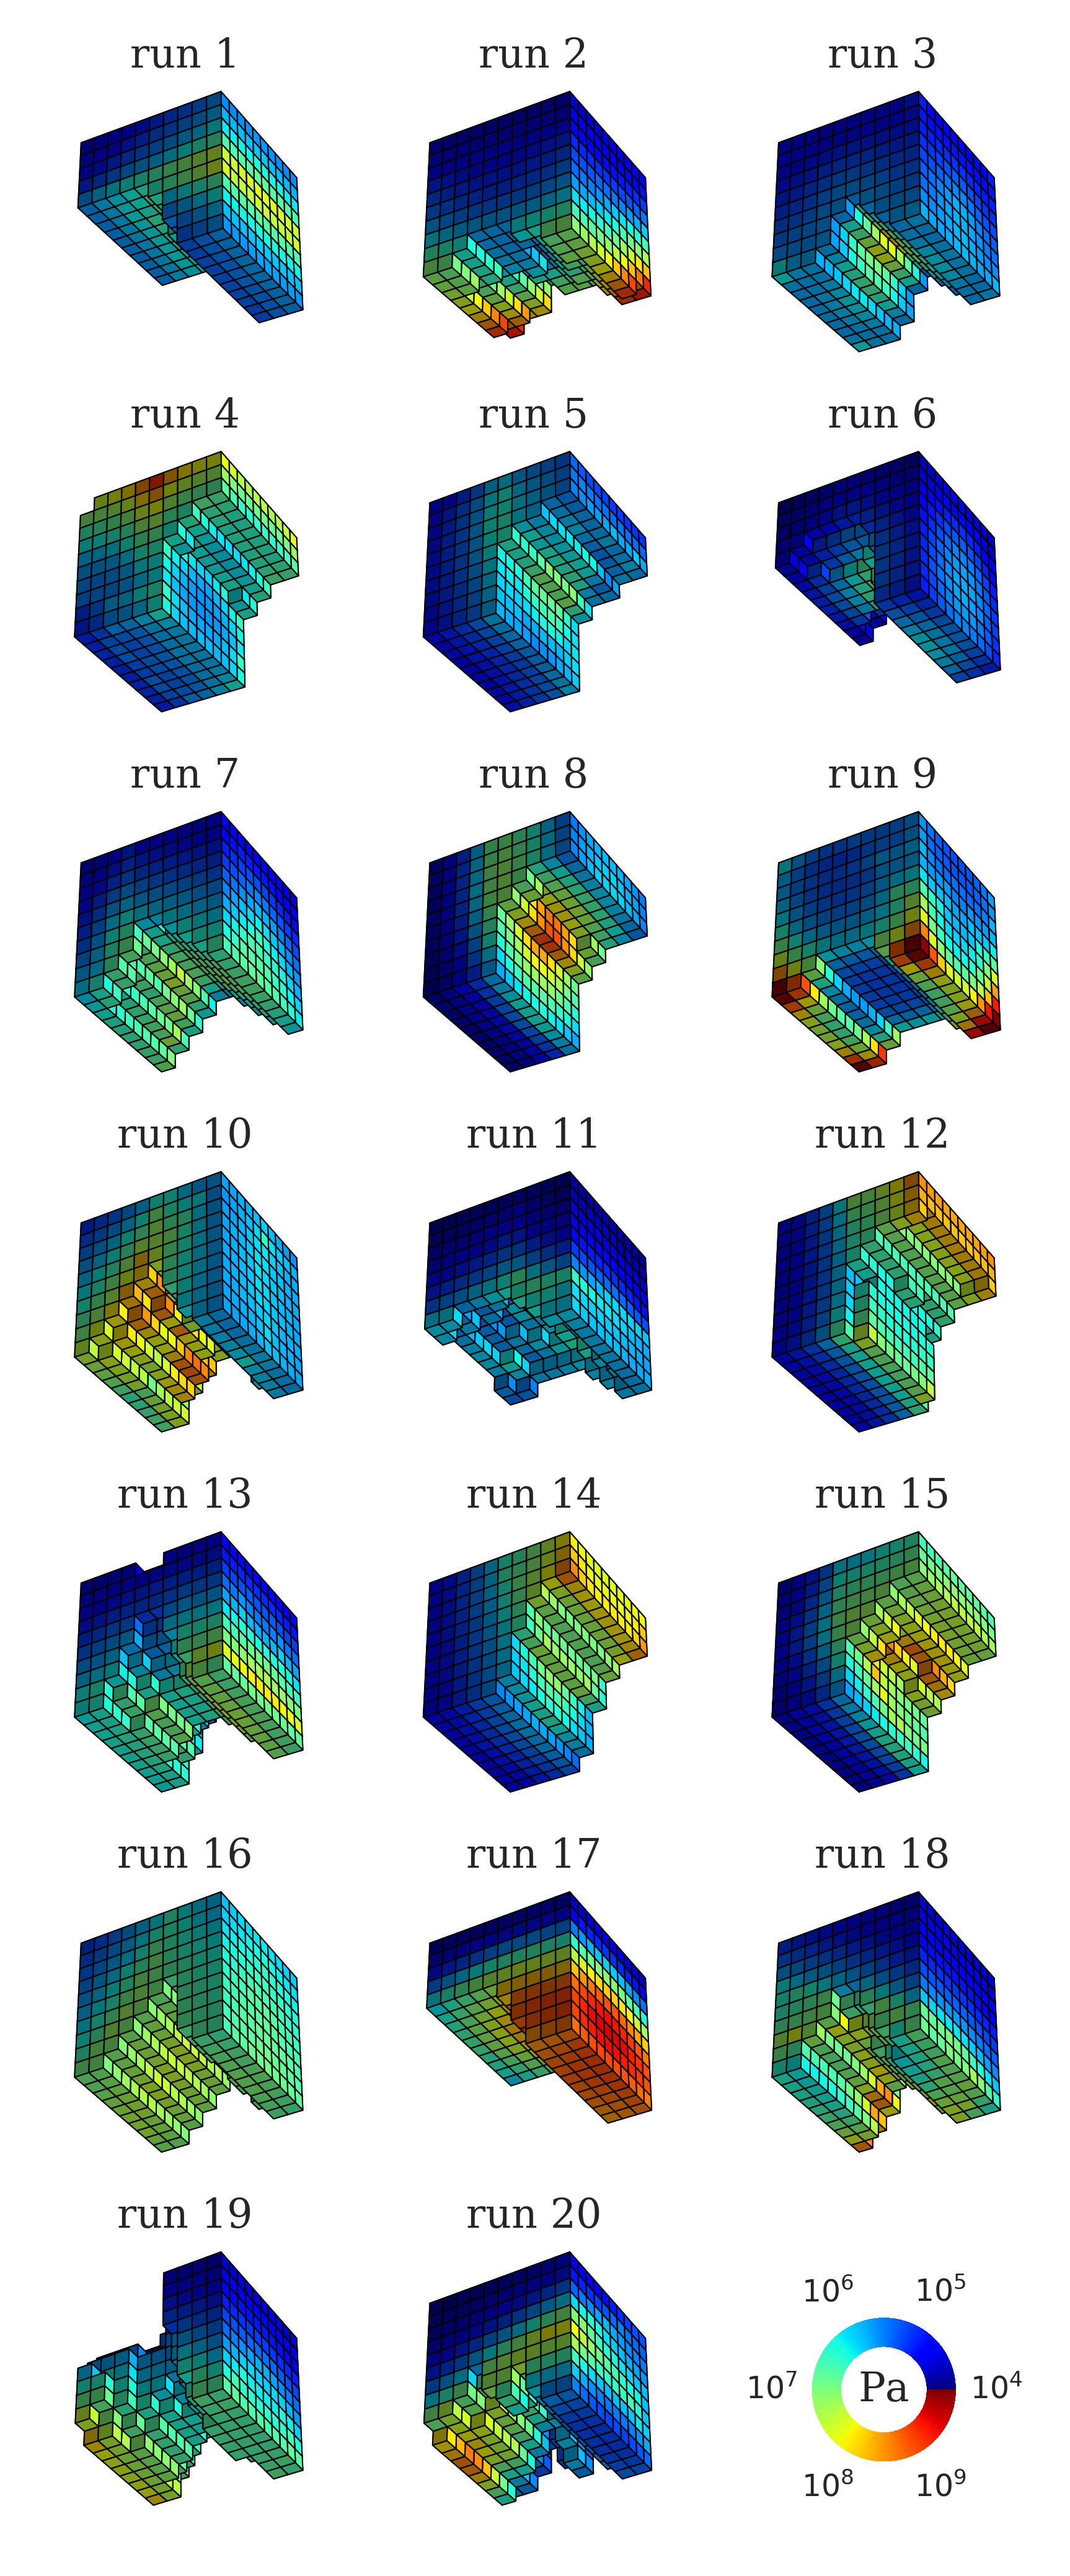
\includegraphics[width=0.5\linewidth]{Chapter06/img/zero_run_champs}
% \vspace{-2.5em}
\caption{\label{fig:none} Run champions colored by congenital stiffness, which ranges from 10\textsuperscript{4} to 10\textsuperscript{10} Pa. After settling under gravity, robots move toward the right-hand side of the page.}
\end{figure}


\begin{figure}%[H]
\centering
{\Large \textbf{Stress-adaptive champions (Eq. \ref{eq:stress})}}
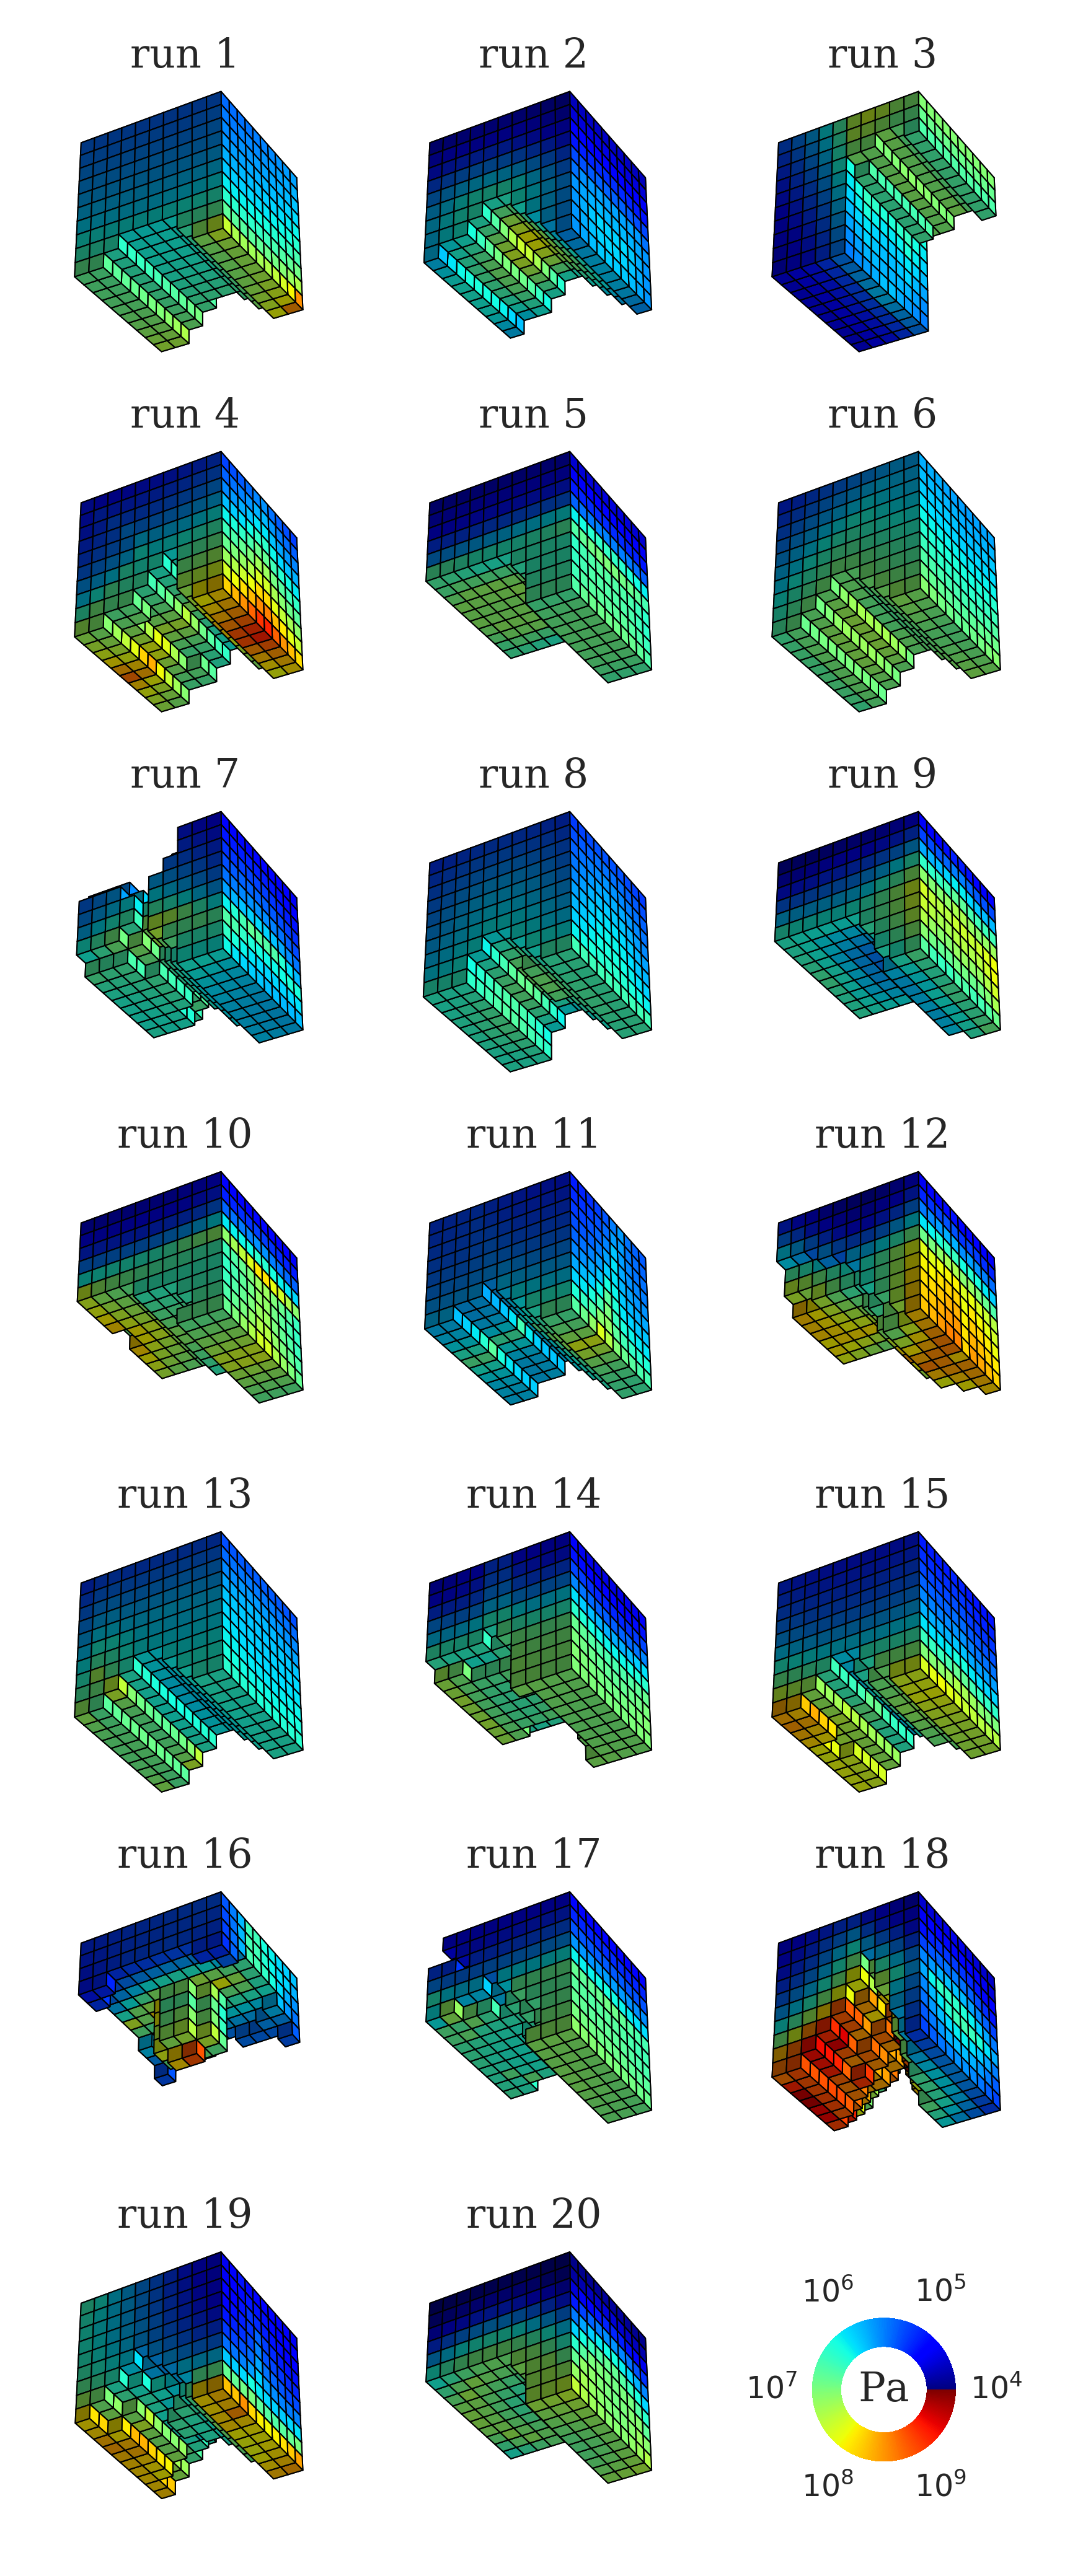
\includegraphics[width=0.5\linewidth]{Chapter06/img/stress_run_champs}
% \vspace{-2.5em}
\caption{\label{fig:stress} Run champions colored by congenital stiffness which can change during operation (ontogeny) in response to \textit{engineering stress.}}
\end{figure}

\begin{figure}%[H]
\centering
{\Large \textbf{Pressure-adaptive champions (Eq. \ref{eq:pressure})}}
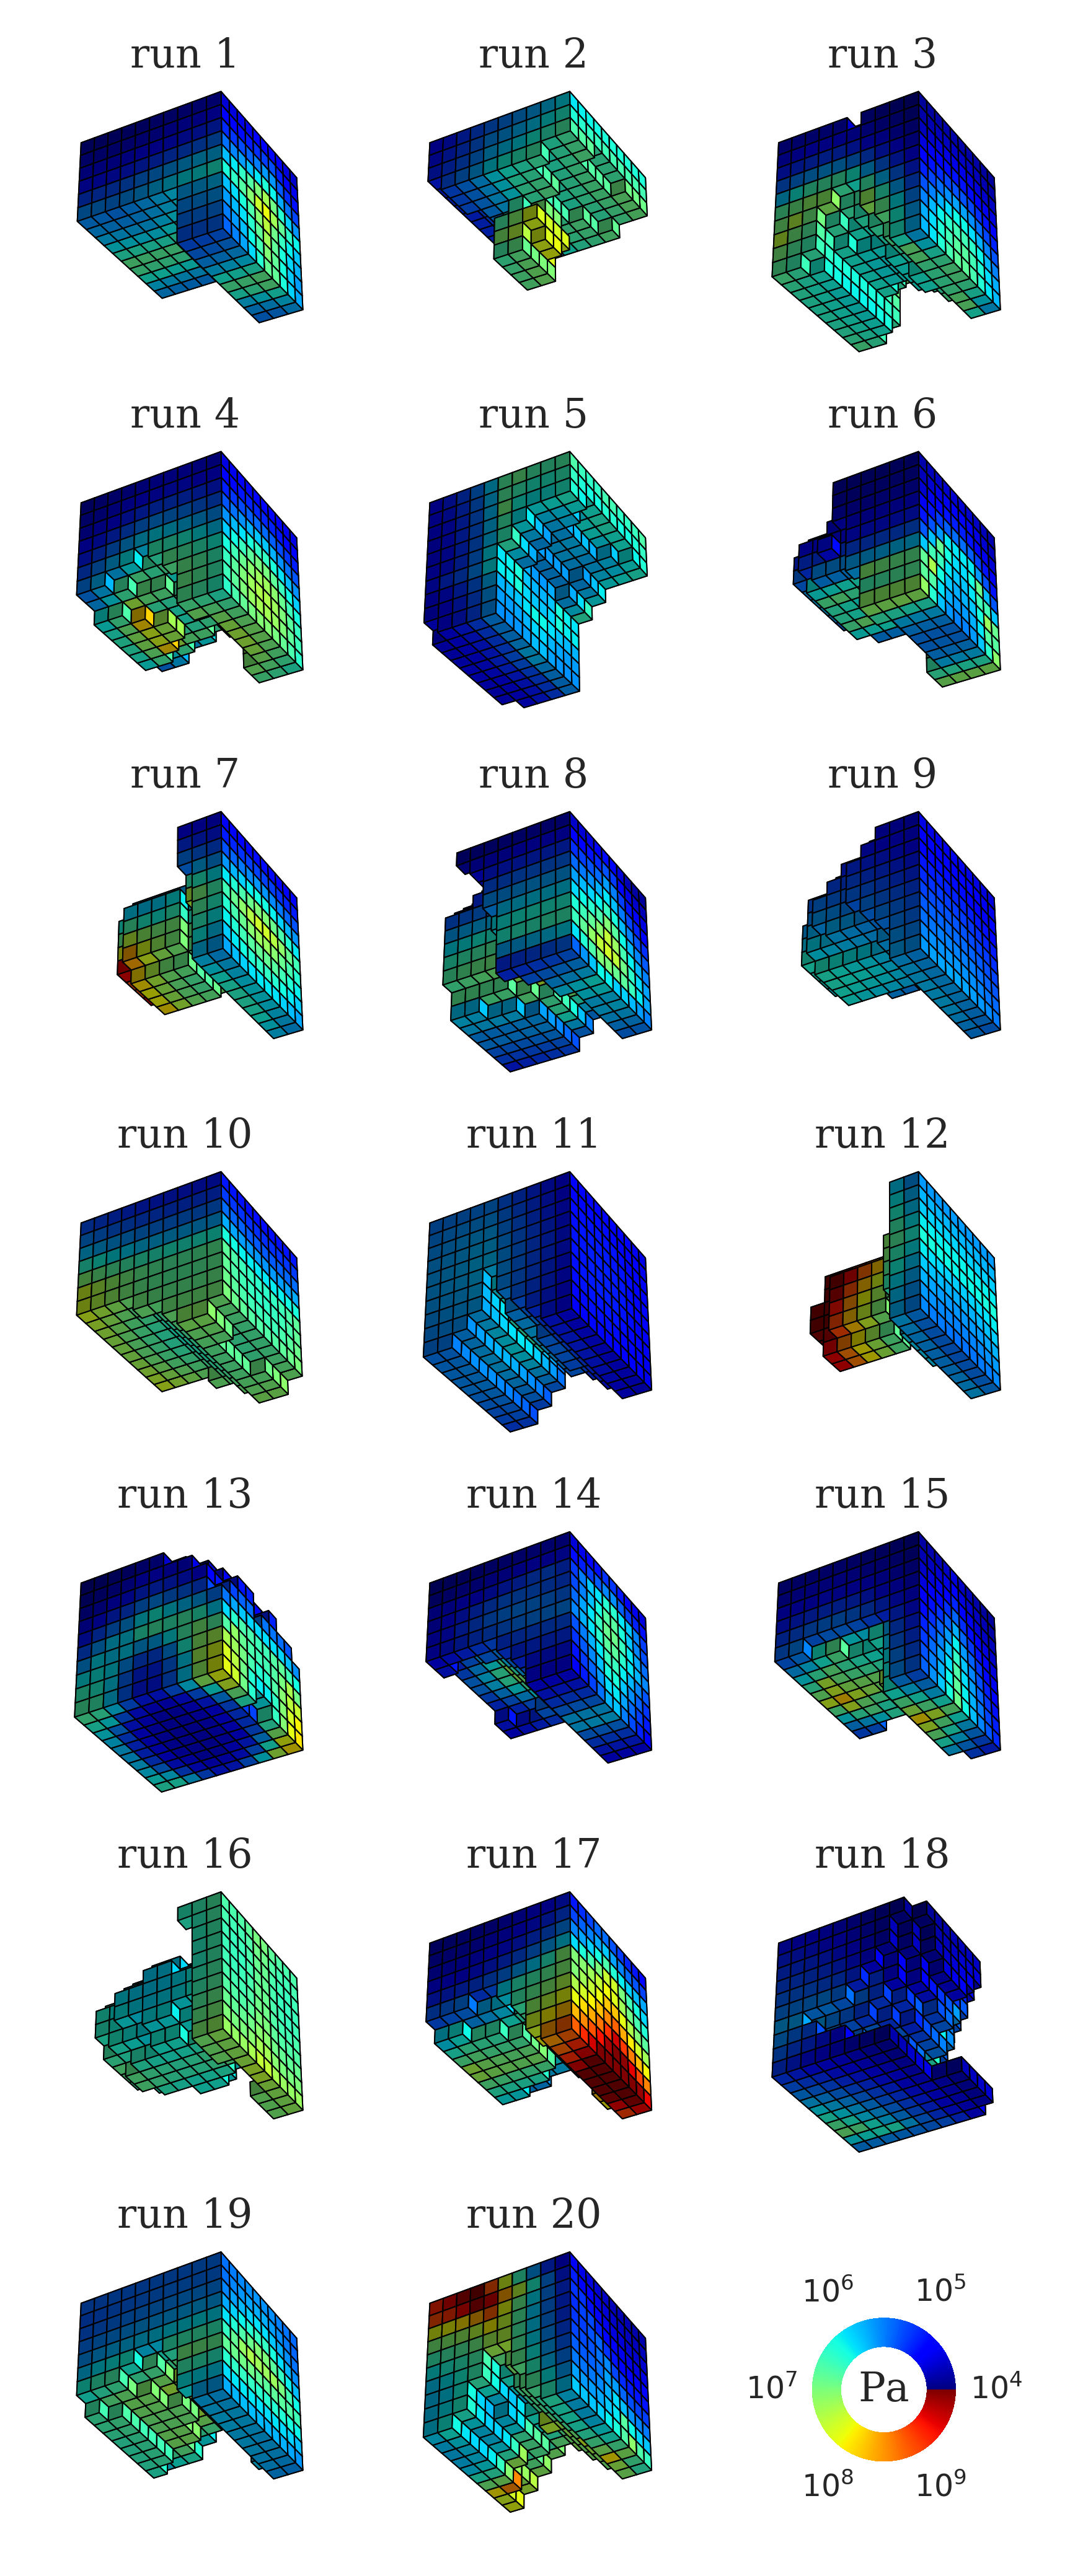
\includegraphics[width=0.5\linewidth]{Chapter06/img/pressure_run_champs}
% \vspace{-2.5em}
\caption{\label{fig:pressure} Run champions are colored by congenital stiffness which can change during operation (ontogeny) in response to \textit{pressure.}}
\end{figure}


\begin{figure*}[t]
\centering 
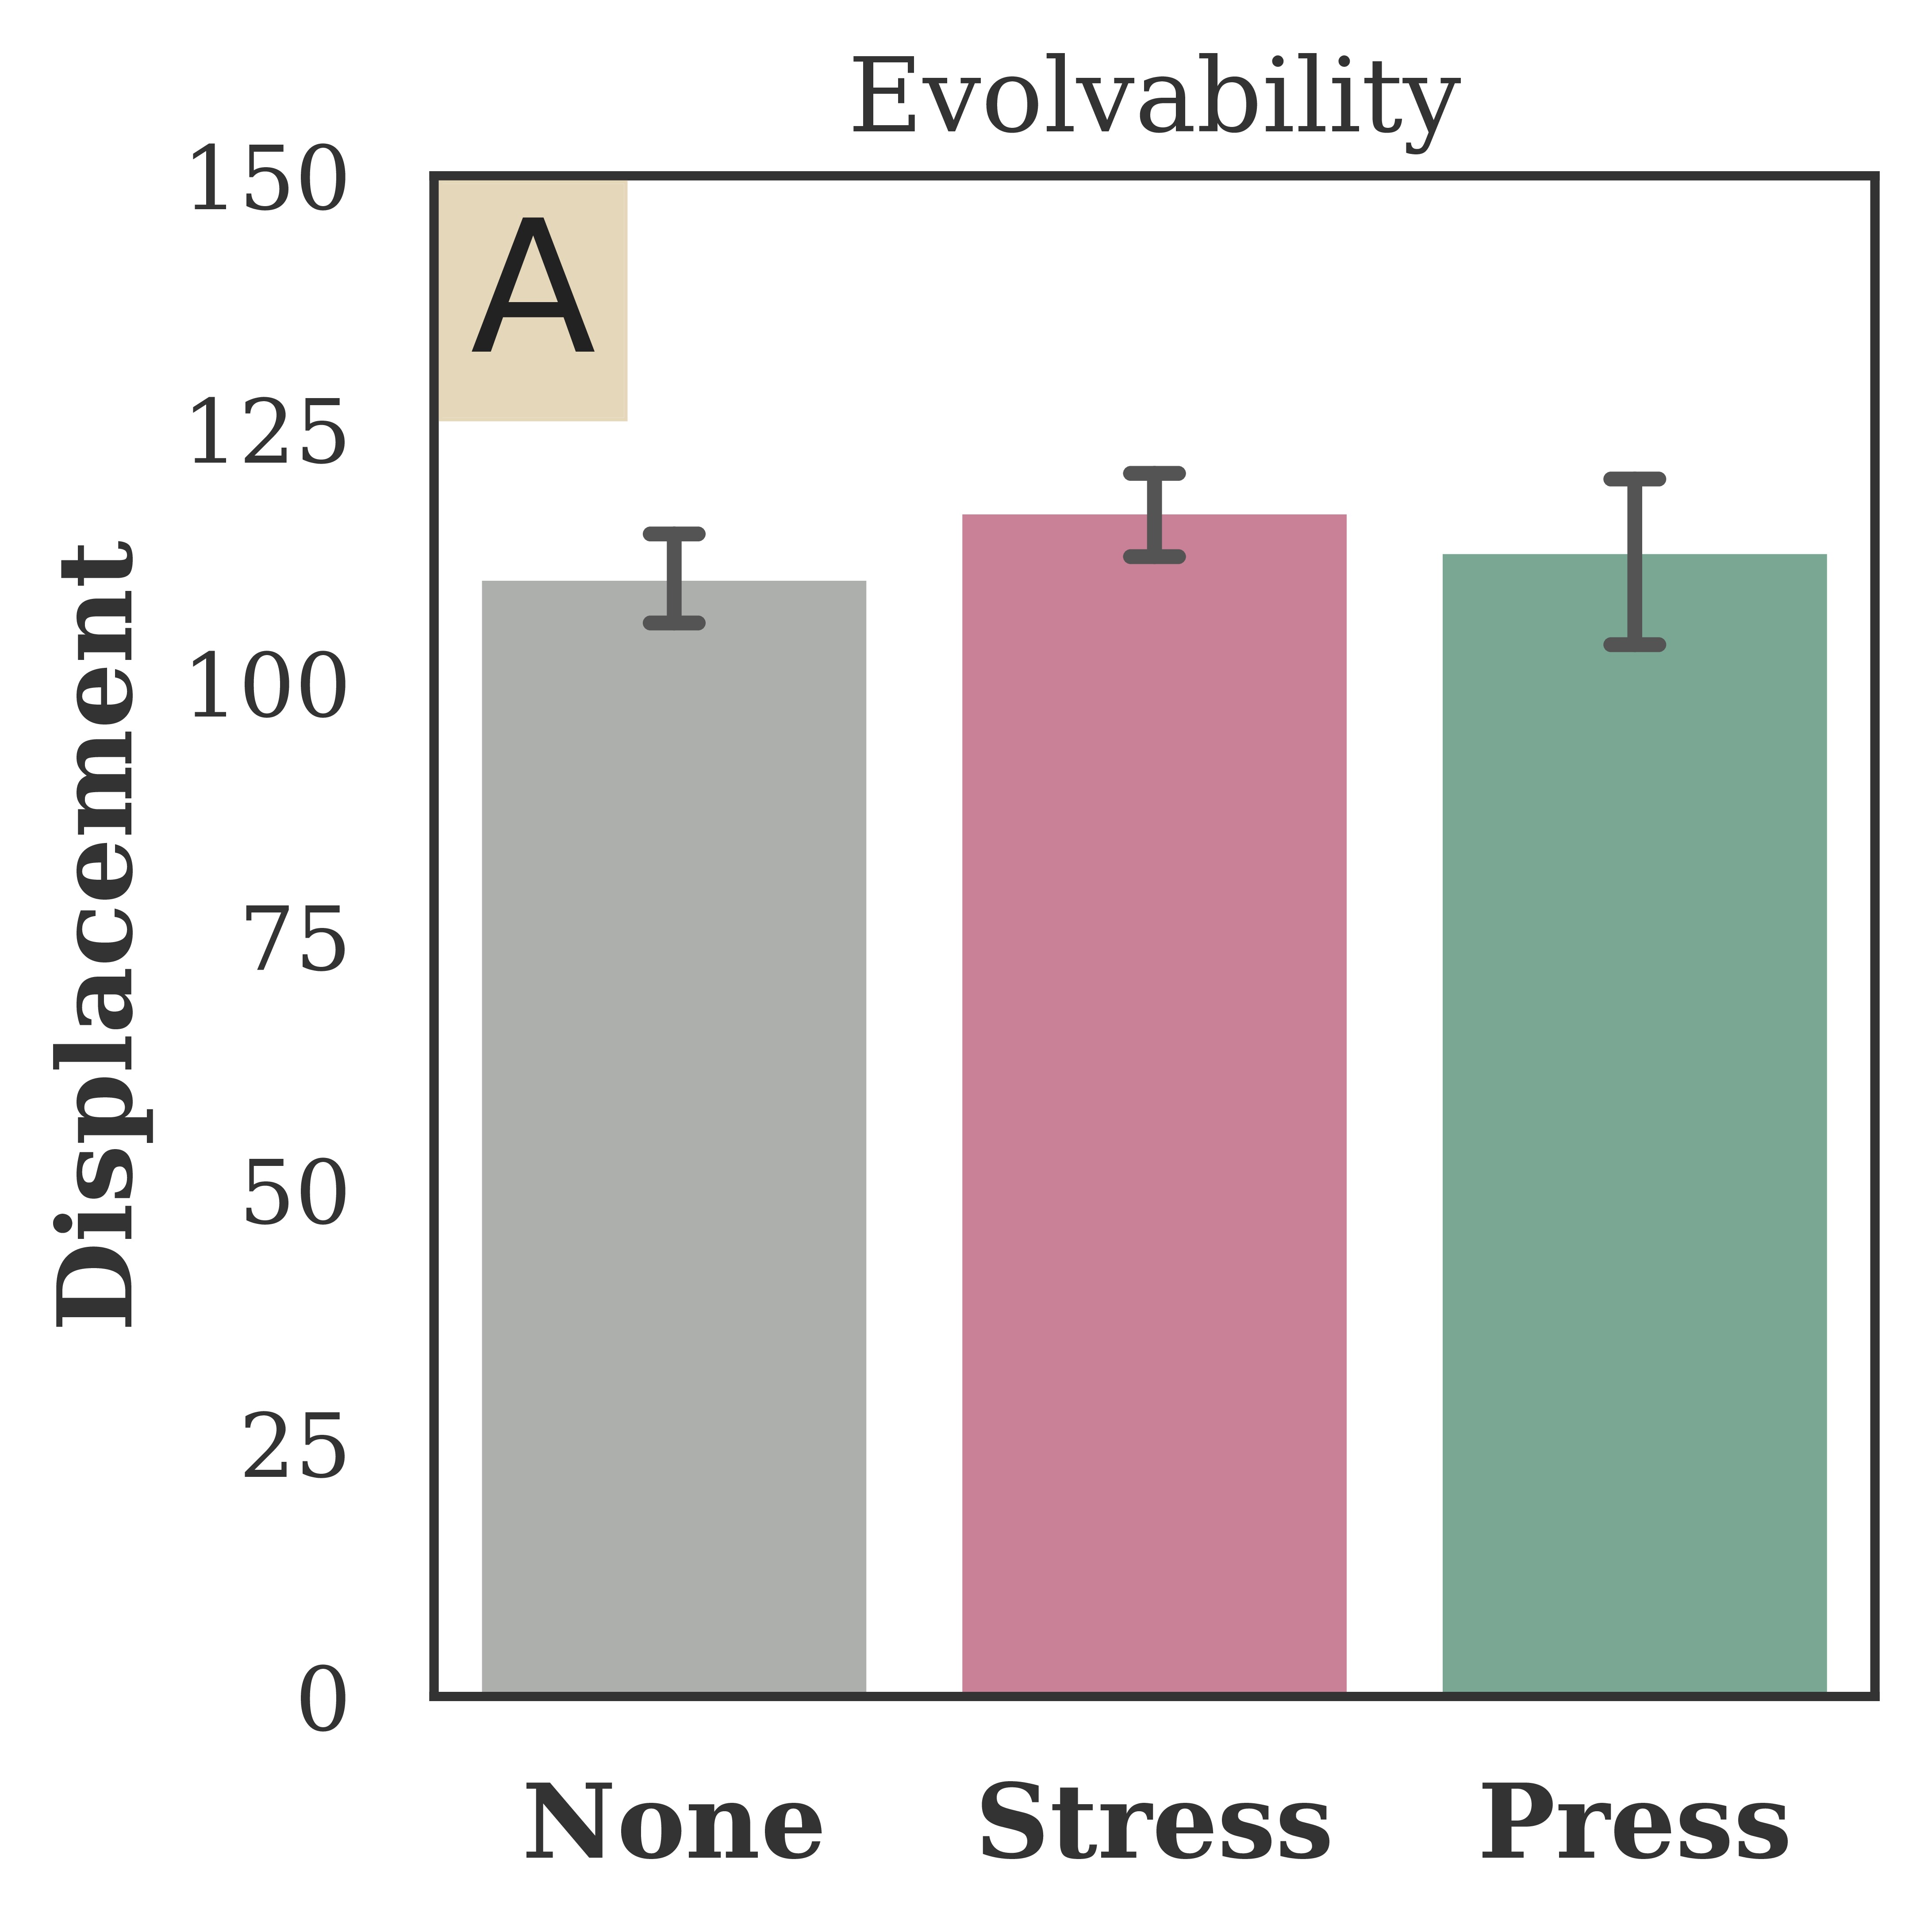
\includegraphics[width=0.32\linewidth]{Chapter06/img/Evolvability}
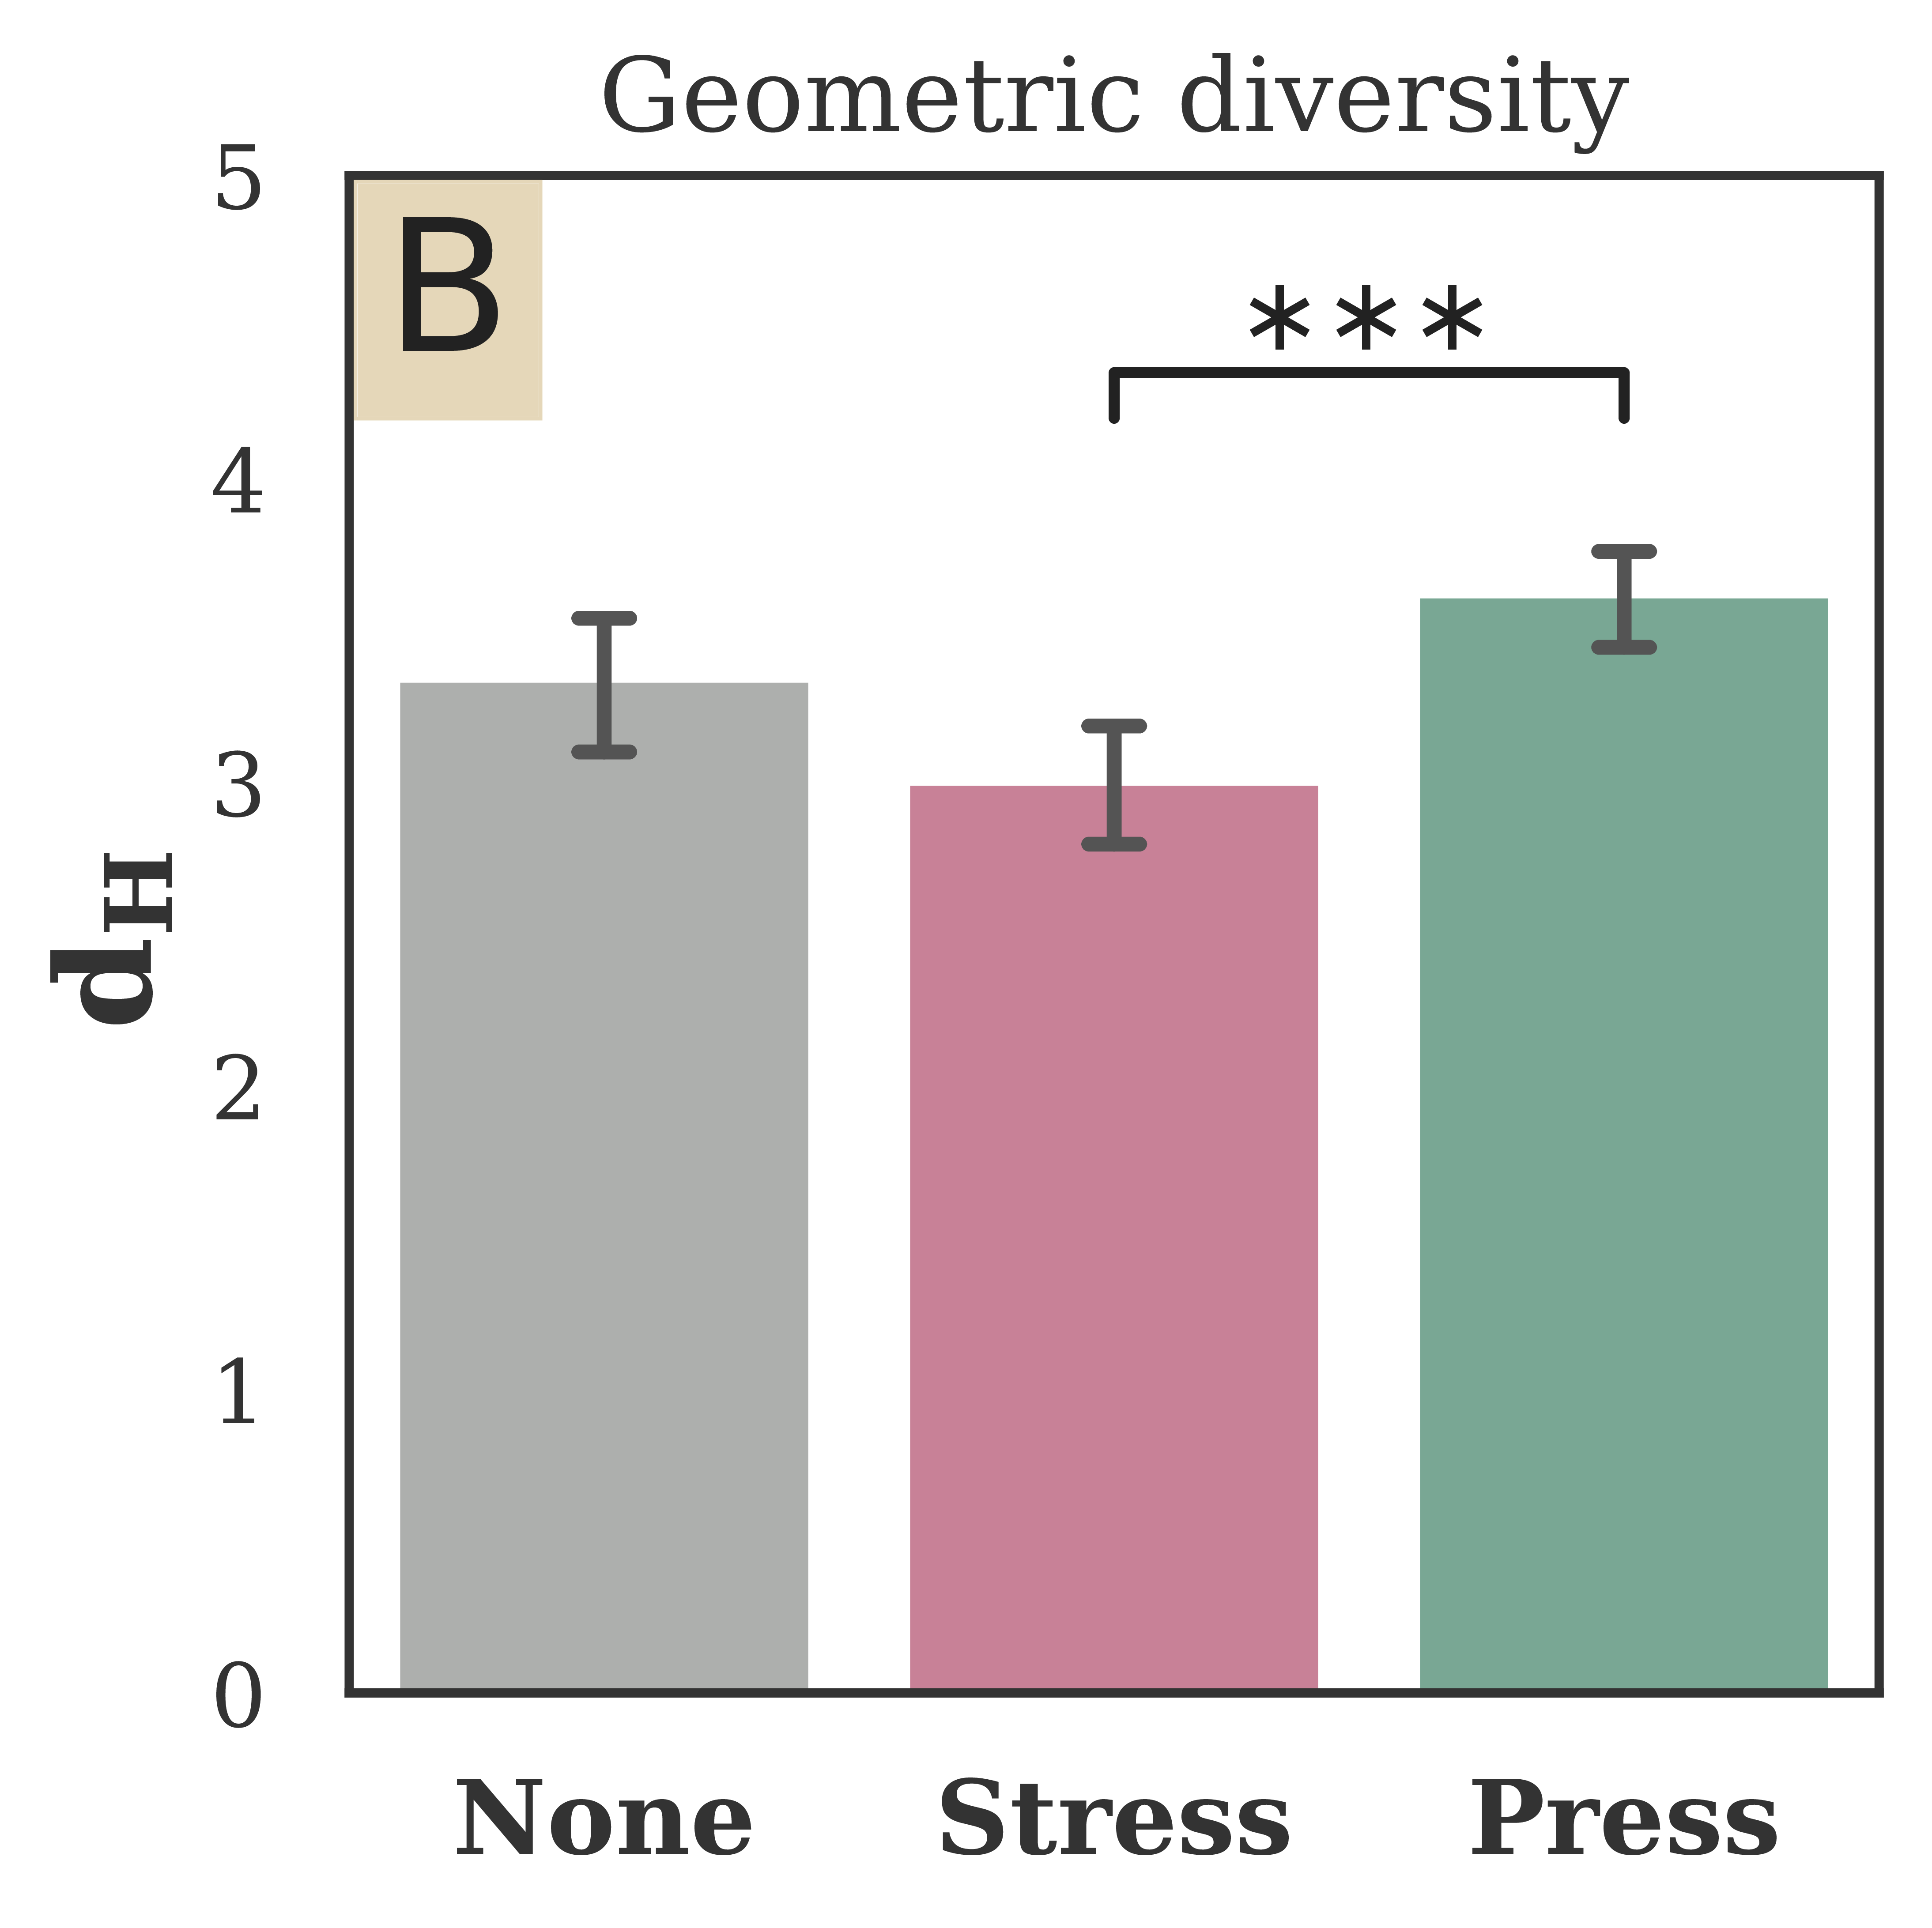
\includegraphics[width=0.32\linewidth]{Chapter06/img/Hausdorff} 
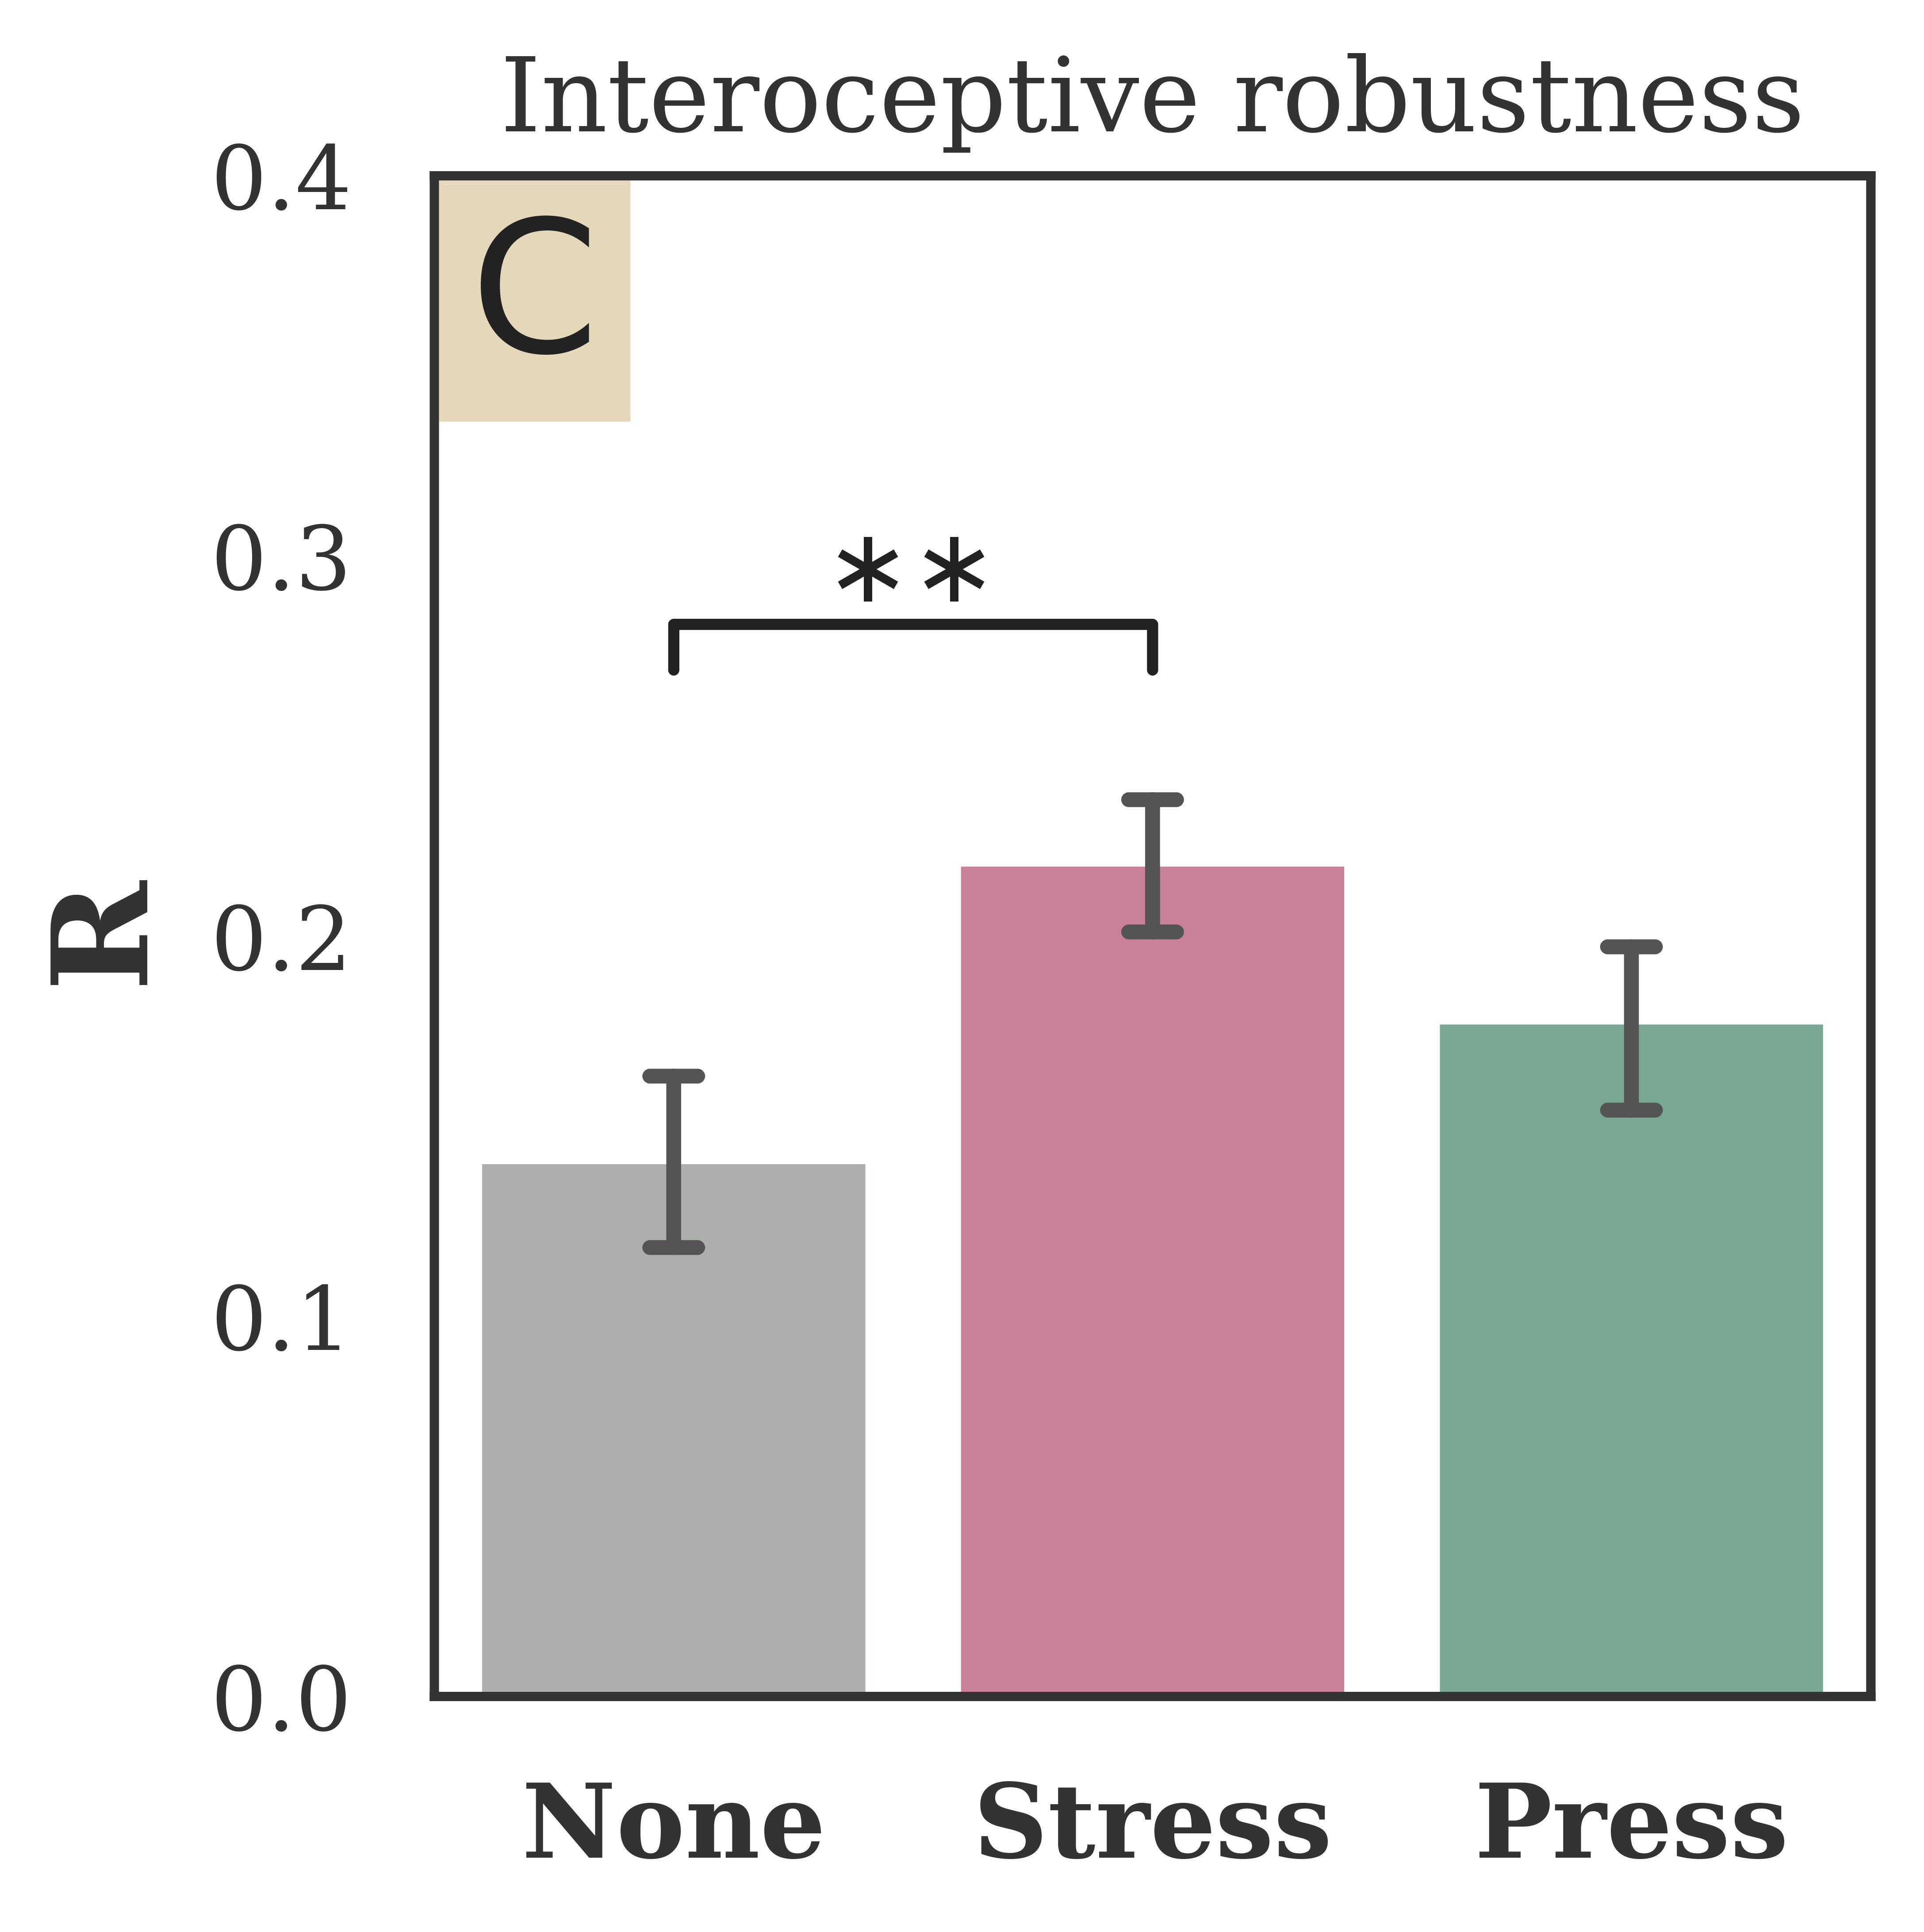
\includegraphics[width=0.32\linewidth]{Chapter06/img/Robustness}
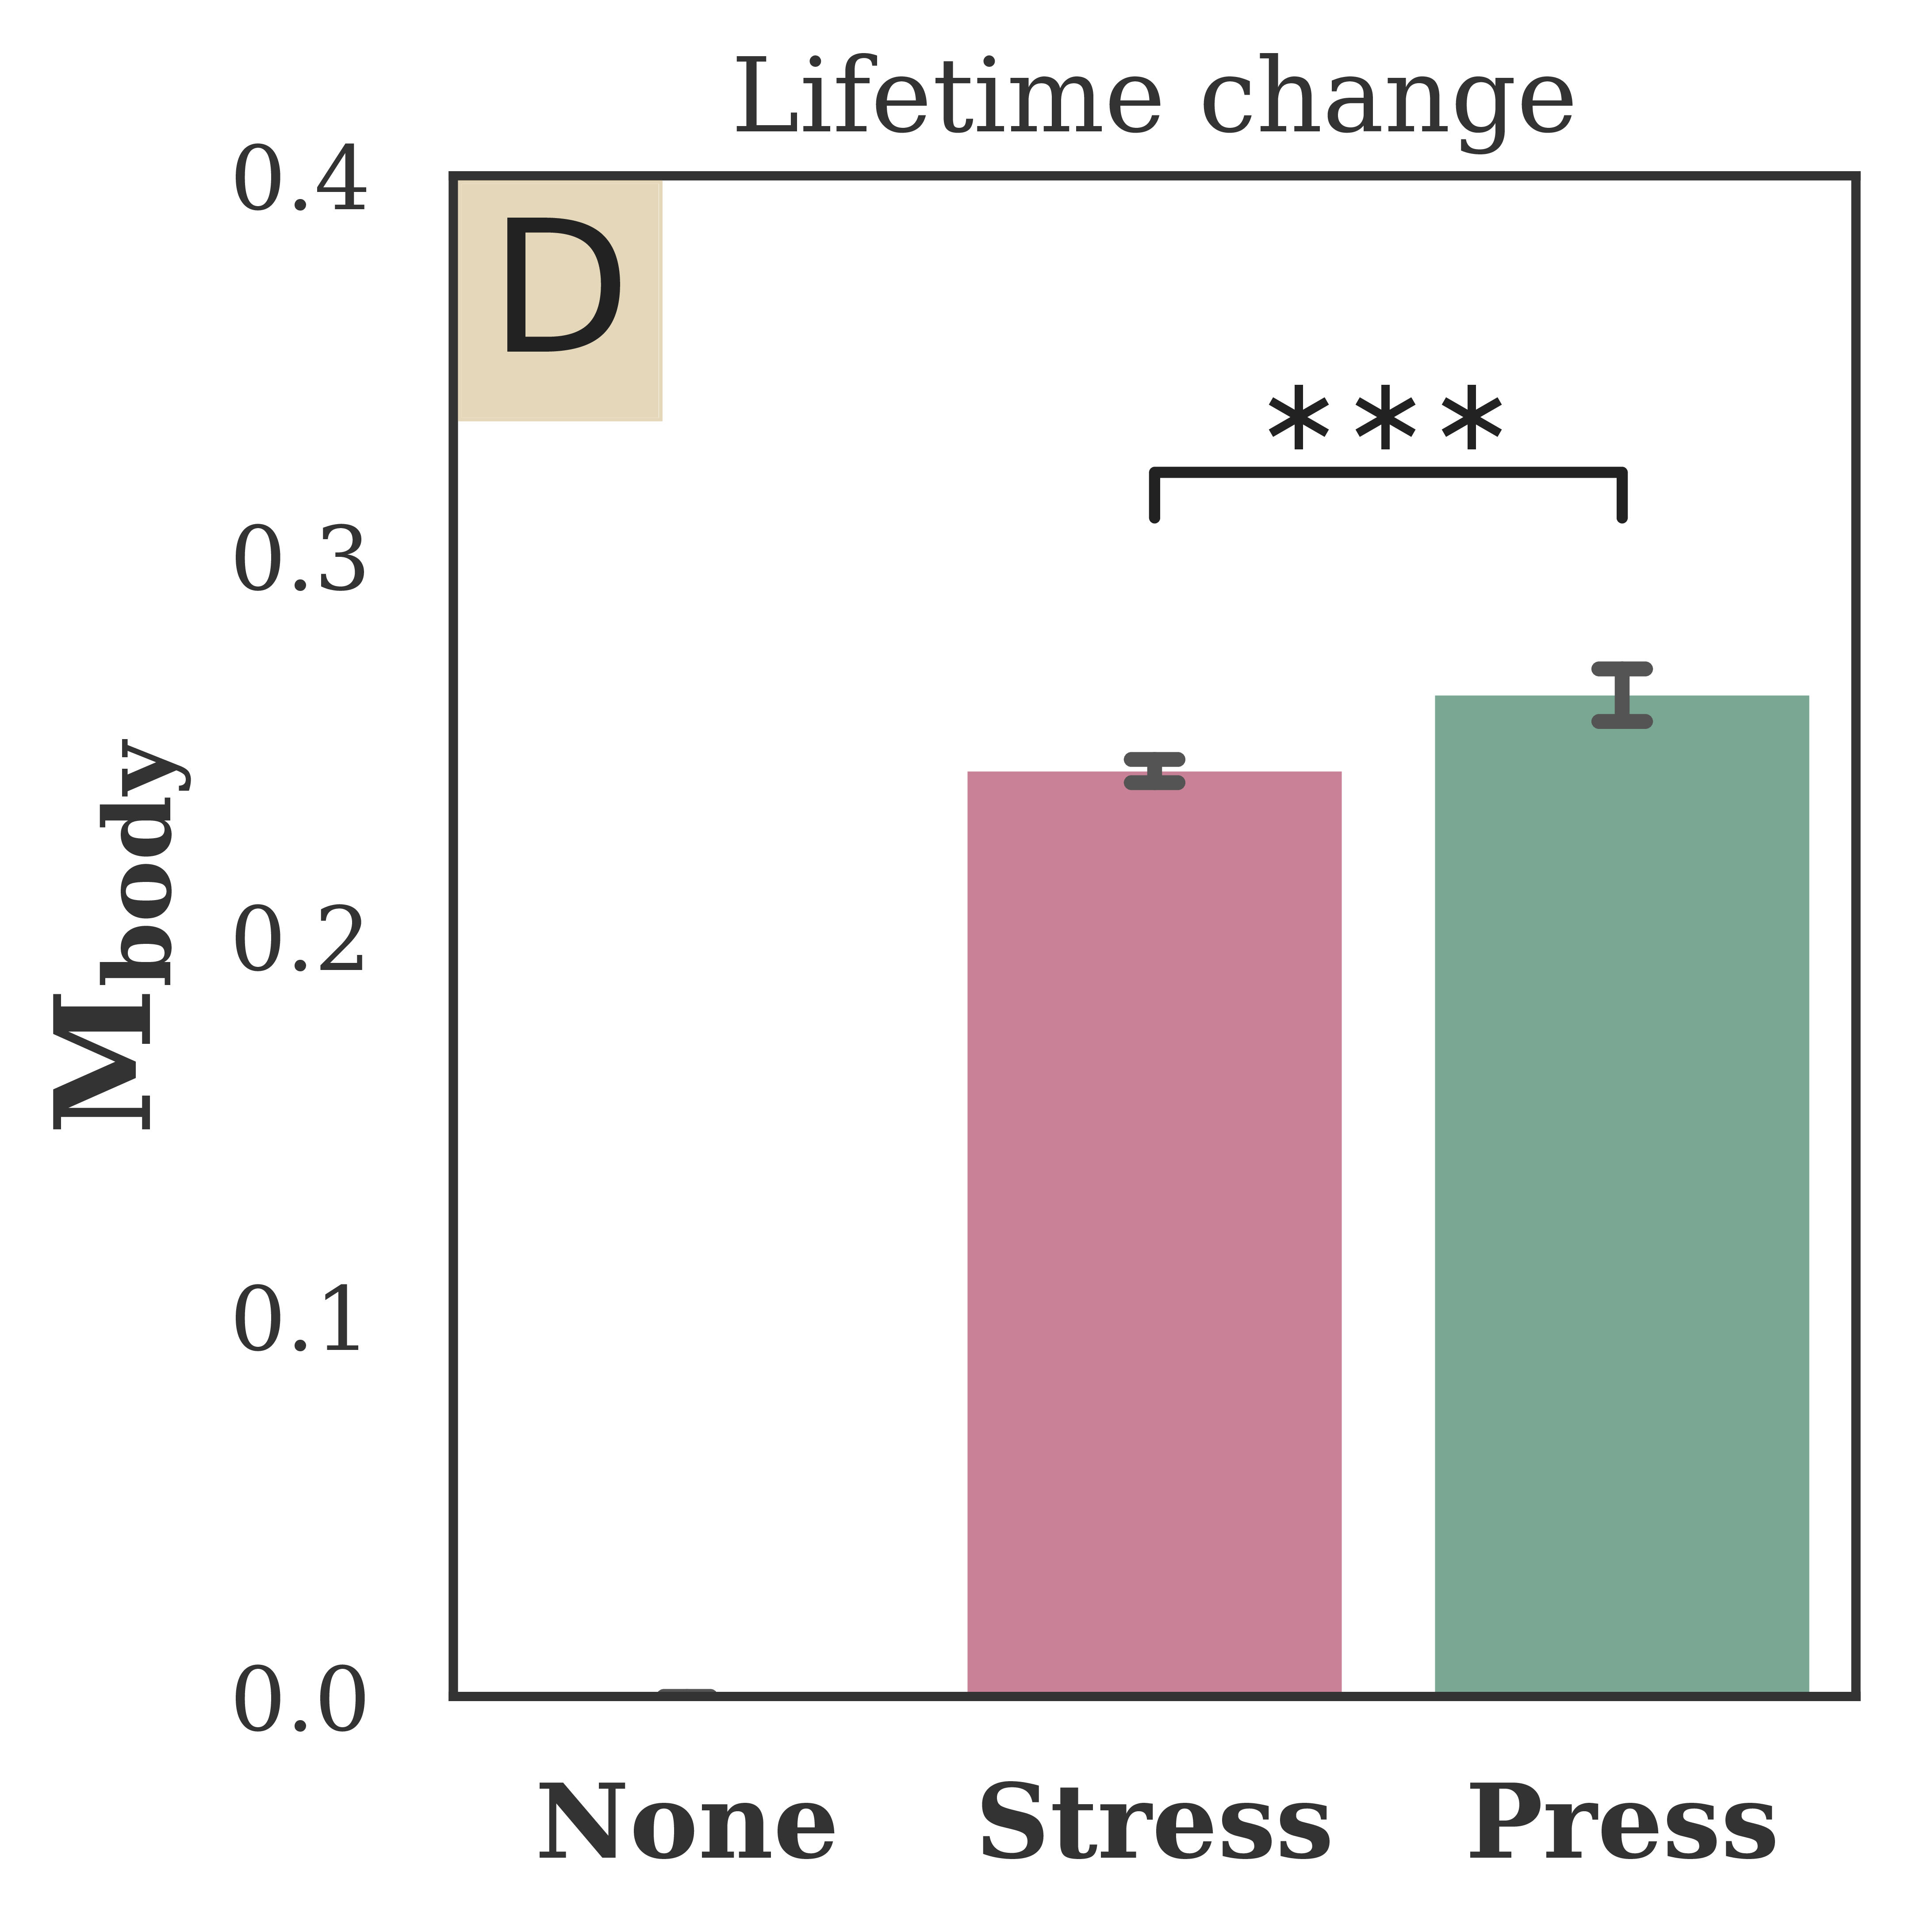
\includegraphics[width=0.32\linewidth]{Chapter06/img/Mean_Change}
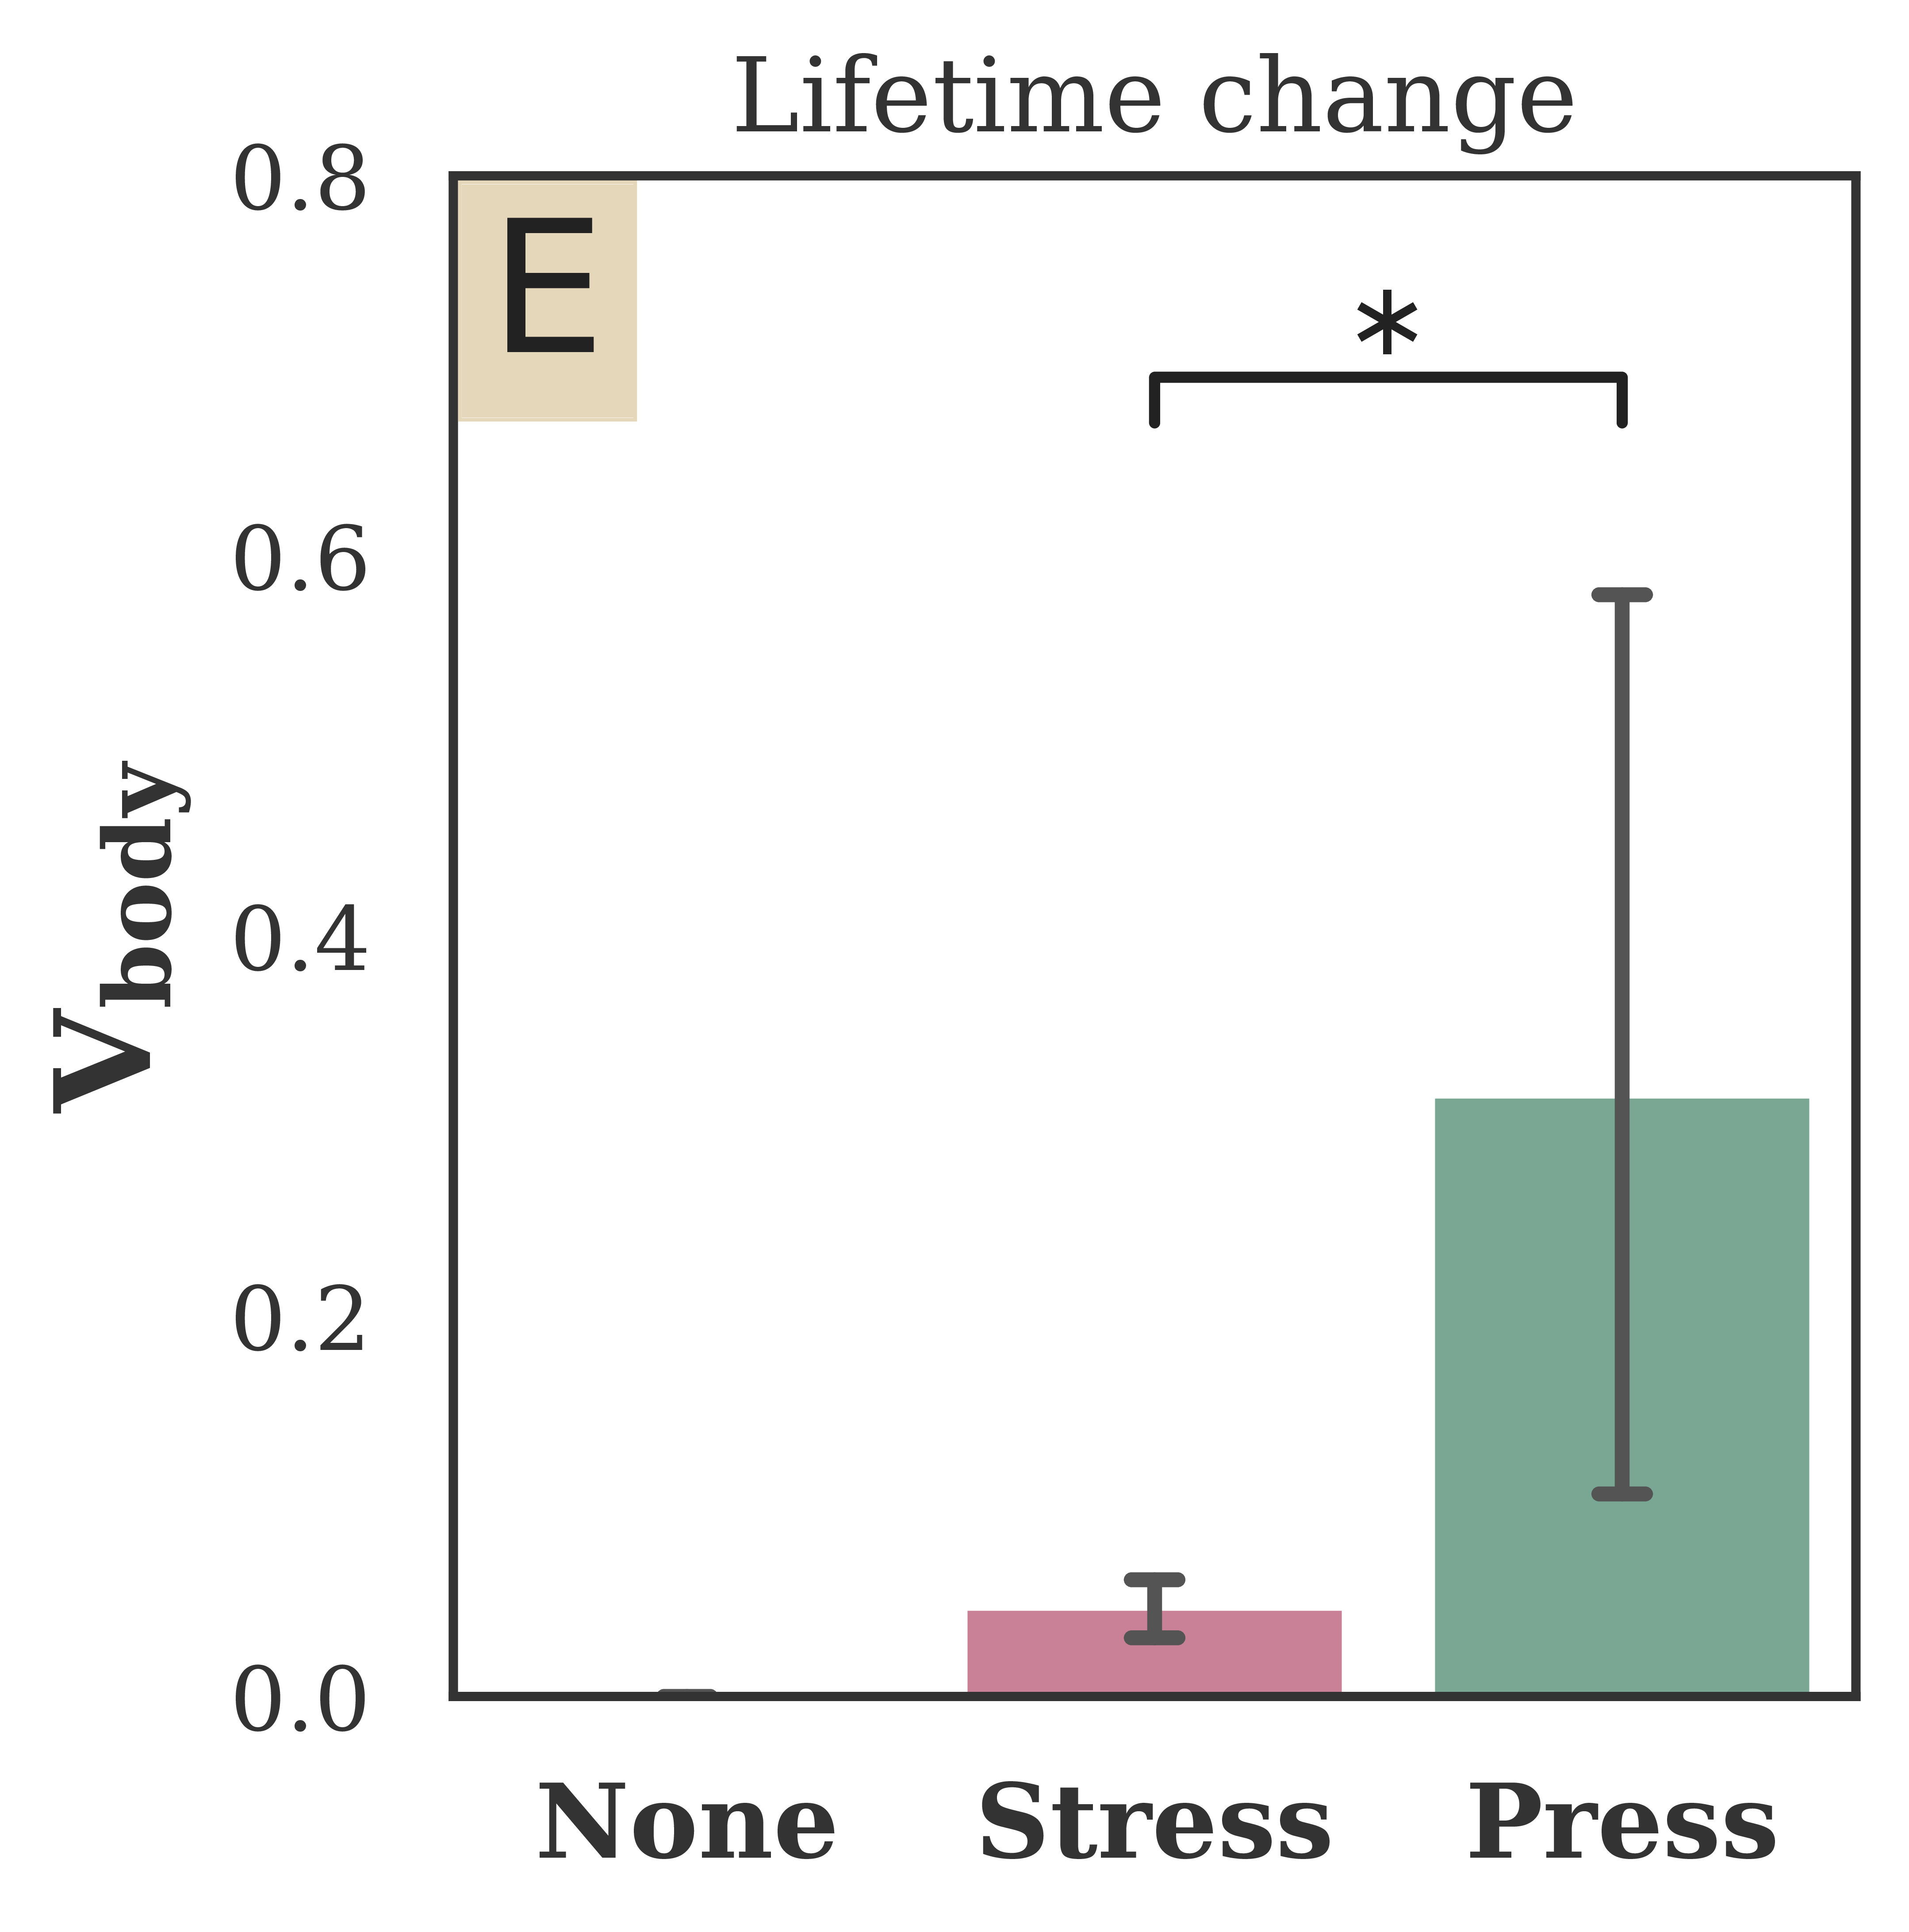
\includegraphics[width=0.32\linewidth]{Chapter06/img/Variance_Change}
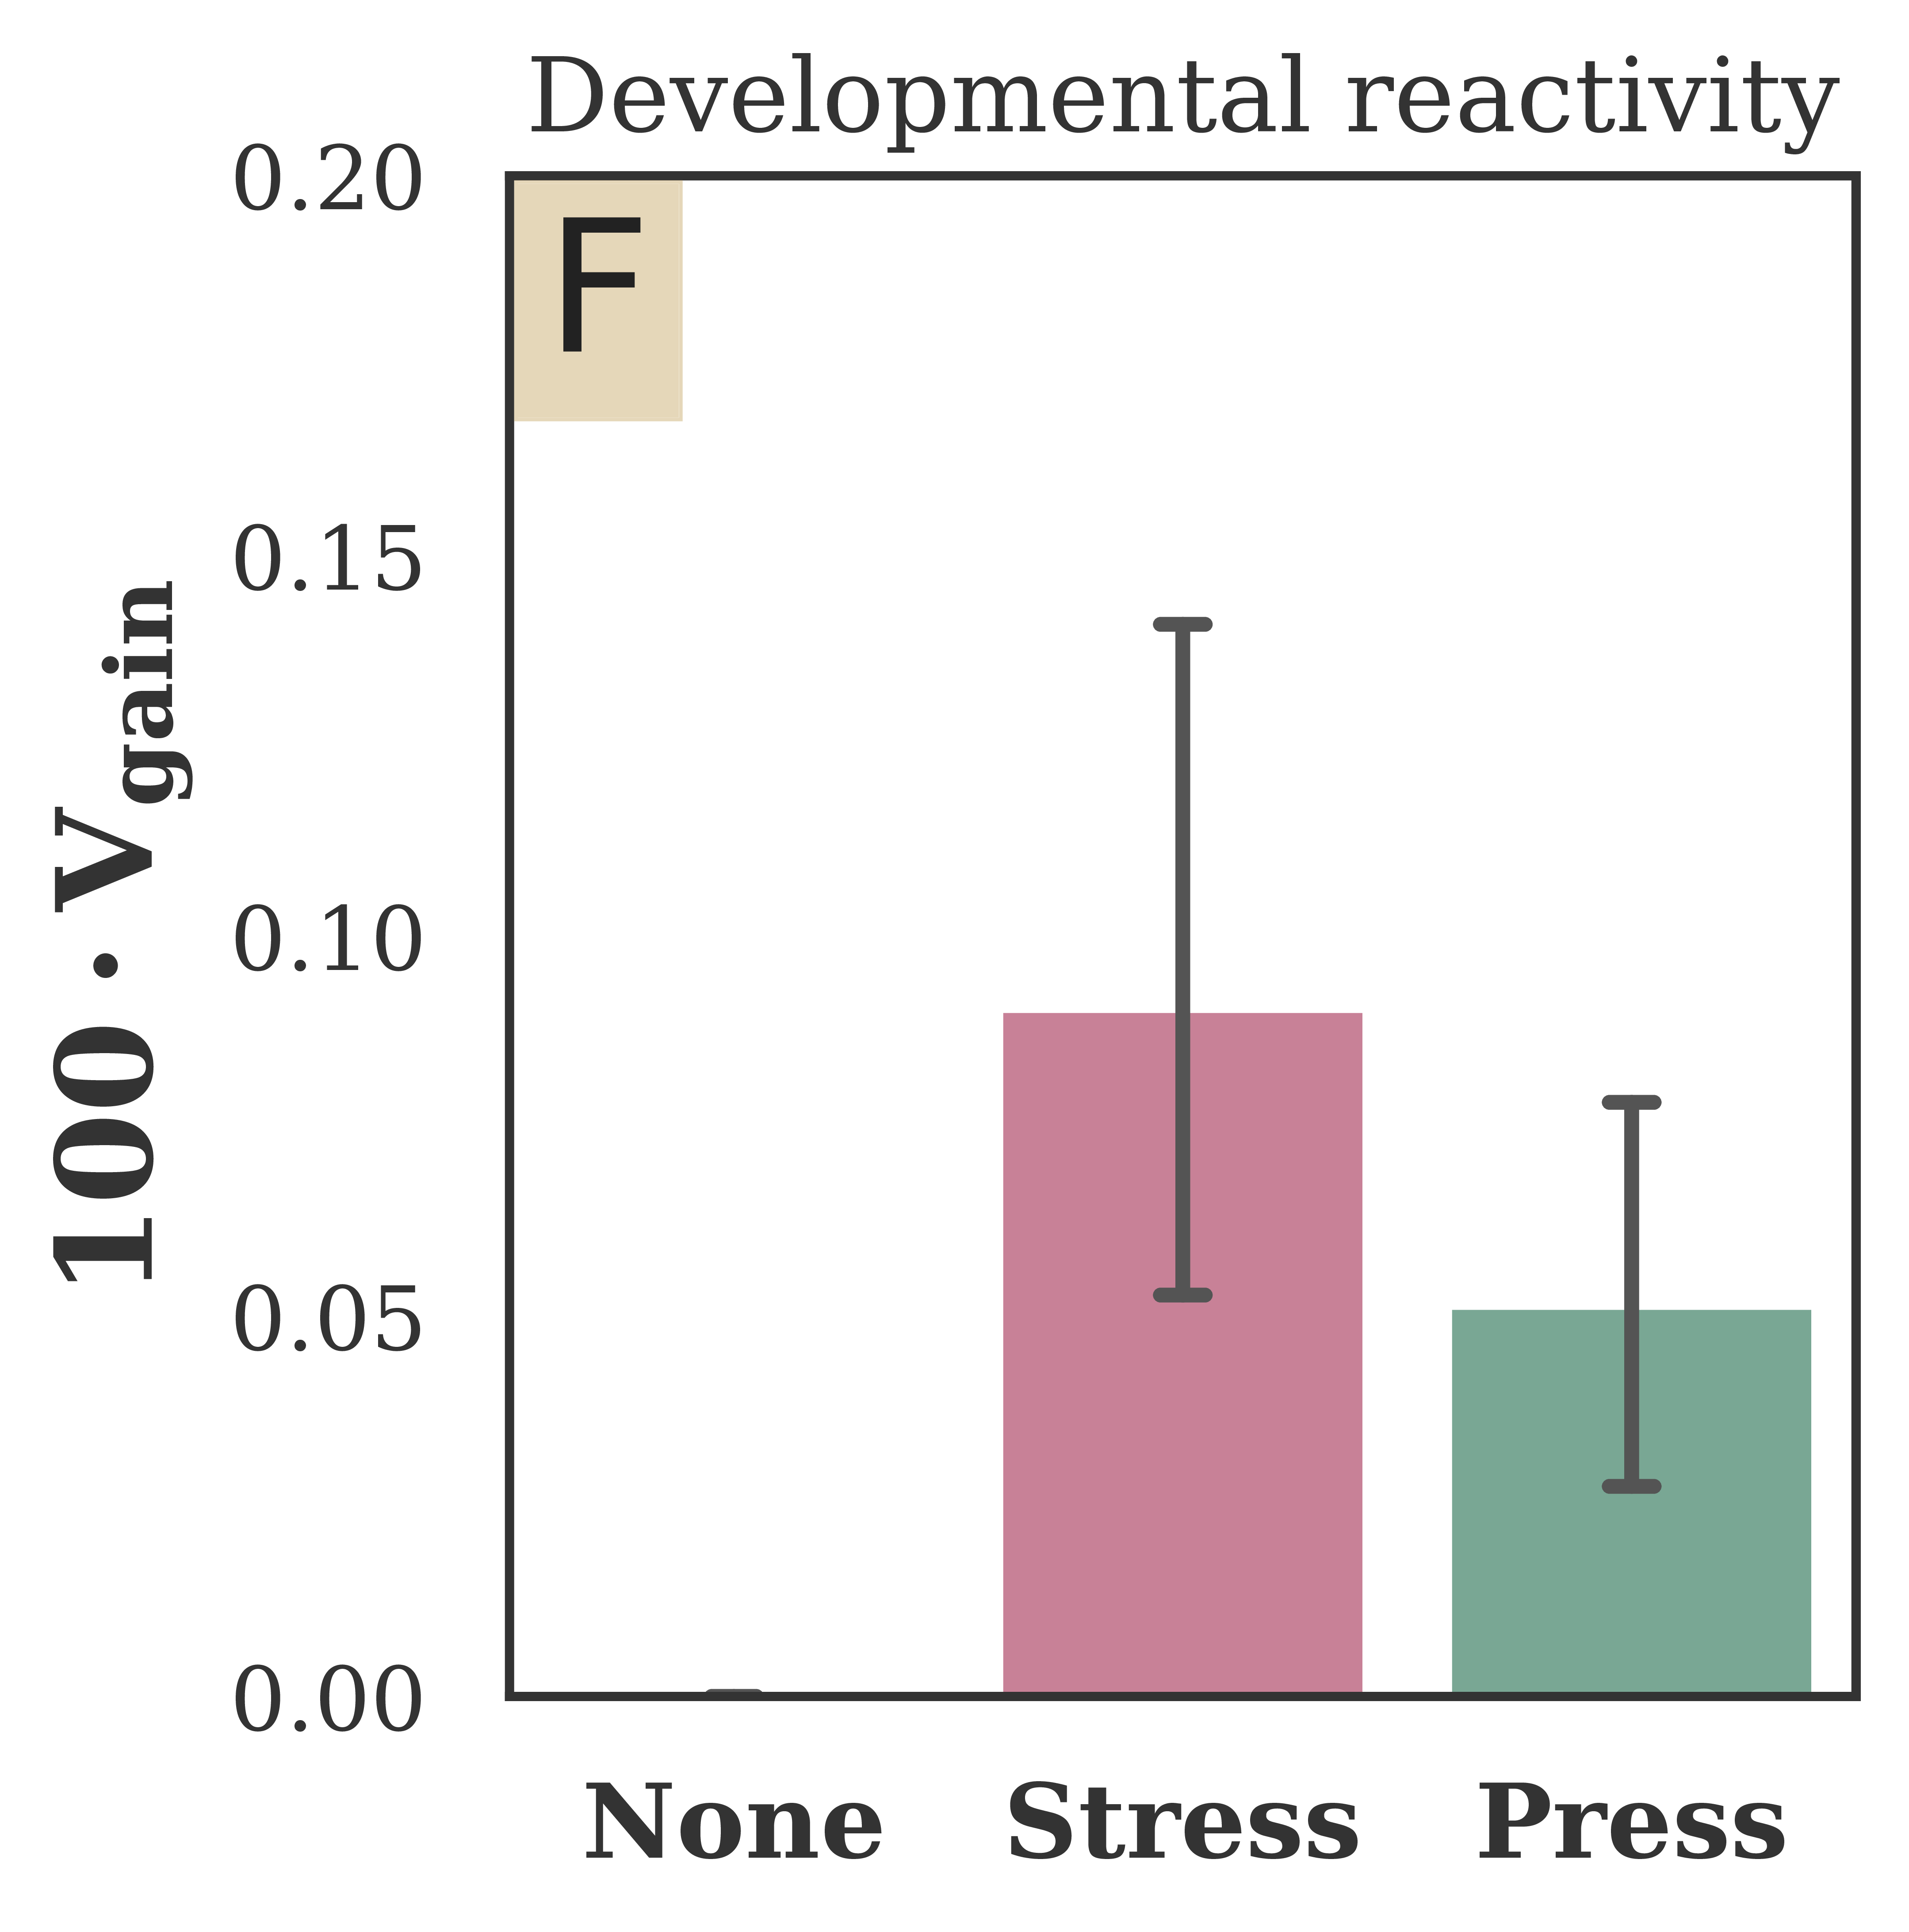
\includegraphics[width=0.32\linewidth]{Chapter06/img/Var_devo_gain}
\caption{\label{fig:run_champs} 
Means (with 95\% C.I.) for various statistics of the run champions, at generation 5000: 
(A) Fitness as the final displacement of a robot, measured by voxel-length units; 
(B) Diversity as the pairwise Hausdorff distances of robot geometries; 
(C) Robustness as the relative fitness (testing fitness divided by training fitness) after development is removed and a random stiffness distribution is introduced
into the champion's body (Eq. \ref{eq:robustness});
(D) Mean, taken across the body, of relative lifetime change in stiffness, as a measure of the lack of canalization (Eq. \ref{eq:mu}; lower bars indicate more canalization);
(E) Variance, taken across the body, of relative lifetime change in stiffness, as a measure of heterogeneity/nonuniformity in developmental reactions (Eq. \ref{eq:sigma});
(F) Variance, taken across the body, of the coefficients/gain of developmental reactivity (Eq. \ref{eq:sigma-gain}).
}
\end{figure*}


\subsection{Geometric diversity.}

We investigate morphological diversity next by
employing the Hausdorff distance $d_H$ as a metric to compare the similarity of two robot geometries, $A$ and $B$.
For each voxel in $A$, the closest voxel in $B$ is identified, according to euclidean distance $d$.
Similarly, for each voxel in $B$, the closest voxel in $A$ is identified.
The Hausdorff metric is the larger of these two distances. 
Formally,
\begin{equation}
\label{eq:hausdorff}
d_H(A,B) = \max\{\,\sup_{a \in A} \inf_{b \in B} d(a,b),\; \sup_{b \in B} \inf_{a \in A} d(a,b)\,\} \, . %\mbox{.}
\end{equation}
Informally, two robots are close in the Hausdorff distance if every voxel of either robot is close to some voxel of the other robot. 
 

We calculated the Hausdorff distance between each of the $\binom{20}{2}=190$ possible pairings of the 20 run champions (Fig. \ref{fig:run_champs}B).
Because $d_H(A,B)$ depends on the orientations of $A$ and $B$, we rotate $B$ in the $xy$ plane (0, 90, 180, and 270 degrees) and the $yz$ plane (0 and 90 degrees), and select the rotation that creates the smallest $d_H(A,B)$.

We found the evolved body shapes of pressure-adaptive robots to be more diverse than those of stress-adaptive robots $(P<0.001)$.
We did not find a significant difference, at the 0.05 level, between adaptive and nonadaptive treatments using this particular measure of morphological diversity.

Across all three treatments,
there appear on visual inspection to be three types of geometries (Figs. \ref{fig:none}-\ref{fig:pressure}): a $\Pi$ robot with wide posterior and anterior legs; a $\Gamma$ robot whose legs meet perpendicularly; and a $\Upsilon$ robot that connects a (mainly cylindrical) leg perpendicularly to the center of a $10\times10$ vertical plane.
Depending on how one counts, the $\Upsilon$ species can be seen in at most one nonadaptive robot (Fig. \ref{fig:none}, run 19), two stress-adaptive robots (Fig. \ref{fig:stress}, runs 7 and 16), and six pressure-adaptive robots (Fig. \ref{fig:pressure}, runs 2, 6, 7, 9, 12, and 16).
Pressure-adaptive robots have more diversity by virtue of more $\Upsilon$ robots.


\subsection{Interoceptive robustness.}

To investigate the relative robustness (if any) across the three treatments,
in the following experiment, development was manually removed from the stress- and pressure-adaptive run champions.
We then tested the sensitivity of the resulting reduced robots to their evolved congenital stiffness distribution (Fig. \ref{fig:run_champs}C).
To do so, we replaced the evolved network dictating material stiffness, $\mathbb{C}_2,$ with a random number generator that draws from the same range of possible stiffness ($10^4 - 10^{10}$ Pa).
That is to say, we `built' the evolved run champions without any errors in the specifications of geometry and actuation, but completely ignored the evolved specifications of their material stiffness, replacing them instead with random noise.
We then calculated the relative fitness
\begin{equation}
\label{eq:robustness}
R = F_{\text{test}}\,/\,F_{\text{train}} \, ,
\end{equation}
where $F_{\text{train}}$ is the fitness achieved using the evolved stiffness and $F_{\text{test}}$ is the fitness when tested with a random stiffness distribution.
We repeated this process ten times for each run champion, each time drawing a new random stiffness distribution.


We found that, compared to nonadaptive robots, reduced stress-adaptive robots 
were 
% are
more robust to this (extreme) discrepancy between training and testing stiffness distributions $(P < 0.01)$.
These results are consistent with the 
found correlation between development and robustness
\cite{miller2004evolving,bongard2011morphological,kriegman2017morphological}.
However, the results here indicate that this correlation is contingent on the kind of environmental
signal the developing agent responds to: there was no difference between pressure-adaptive and nonadaptive robots in this regard, at the 0.05 level.

This implies that by behaving interoceptively with respect to engineering stress, robots evolved the ability to ameliorate large deviations from their expected material properties, but by behaving interoceptively with respect to pressure, robots did not evolve this character.
Because development was manually removed beforehand, robustness in our case was not a matter of changing one's body, as in the example of plant growth \citep{sultan2000phenotypic}; rather, it is an intrinsic property of structure (geometries and actuation patterns) educed from ancestors who changed in response to one particular internal state (stress), but not from those who responded to another (pressure).


The difference in robustness between nonadaptive robots and stress-adaptive, but not pressure-adaptive robots, could be due in part to the fact that there are simply more pressure-adaptive $\Upsilon$ robots than stress-adaptive $\Upsilon$ robots.
While $\Upsilon$ robots tend to be more fit than $\Pi$ and $\Gamma$ robots $(P_{\Pi}<0.05;\, P_{\Gamma}<0.05)$,
they also appear to exploit their material properties to a greater degree, and are thus more sensitive to changes in its constitution, compared to $\Pi$ and $\Gamma$ robots $(P_{\Pi}<0.05;\, P_{\Gamma}<0.01)$.

The $\Upsilon$ robot generates movement by pushing off its posterior leg,
which must be rigid enough to support itself as well as 
propel forward the center portion of its anterior wall 
(e.g.~run 12 in Fig.~\ref{fig:pressure}).
The robot loses kinetic energy, which is stored as elastic strain energy in the spring-like voxels between the wall's center and edge.
The most strain is present in the dorsal portion of the anterior wall.
The springs recoil, restoring kinetic energy and generating forward motion.
If the posterior leg is too soft, or the dorsal anterior wall too rigid, the $\Upsilon$ robot can suffer a large drop in performance.

Differences in geometry, however, shed no light on why (the reduced) stress-adaptive robots are more robust than nonadaptive robots:
the level of significance $(P<0.01)$ does not change after removing the only nonadaptive robot that could possibly be classified as $\Upsilon$ (Fig. \ref{fig:none}, run 19). 
Thus we continue our investigation by analyzing how stress and pressure might differentially affect the rate of developmental reactions.


\subsection{Canalization.}

% According to Waddington \citep{waddington1942canalization}, 
% \begin{quote}
% developmental reactions \textit{as they occur in organisms submitted to natural selection}, are in general canalized. That is to say, they are adjusted so as to bring about one definite end-result regardless of minor variations in conditions during the course of the reaction.
% \end{quote}
One indication of canalization \citep{waddington1942canalization,kriegman2017morphological} in our system is given by the magnitude of $\alpha_i$ in each voxel, as defined by Eqs. \ref{eq:stress} and \ref{eq:pressure}.
However, this is but one of two necessary ingredients for a developmental reaction: it indicates bodywide responsiveness to \textit{potential} stimuli, but ignores the \textit{actual} stimulus.

Thus, as proxy for canalization, we measured the amount of morphological change in reaction to local stimulus, during evaluation.
More precisely, we recorded the mean, across the body, of relative lifetime change in stiffness
\begin{equation}
\label{eq:mu}
M_{\text{body}} = \frac{1}{\#\gamma} \sum_{i \in \gamma} \left| k_i^{+}/k_i^{\circ}-1 \right| ,
\end{equation}
where 
$k_i^{\circ}$ 
is the congenital stiffness,
$k_i^{+}$ is the final stiffness, and
$\gamma = \{i : g_i = 1 \}$ contains the coordinates $i$ of each voxel $g_i$ present in the (bit array) geometry which has cardinality $\#\gamma$ (total voxels). 
Less change---lower $M_{\text{body}}$---indicates more canalization.

On average, voxels in stress-adaptive robots change their relative stiffness less than voxels in pressure-adaptive robots $(P<0.001)$ (Fig. \ref{fig:run_champs}D).
In other words, developmental reactions are canalized to a greater extent in stress-adaptive robots.
It follows, then, that the treatment with increased robustness was also the treatment with increased canalization.

To get a sense of the consistency of developmental reactions, as they occur \textit{across the body} of evolved robots, we also recorded the spatial variance of this relative lifetime change 
\begin{equation}
\label{eq:sigma}
V_{\text{body}} = \text{Var}_{i \in \gamma} \left(\,\left| k_i^{+}/k_i^{\circ}-1 \right|\,\right) .
\end{equation}
By this measure, stress-adaptive robots exhibit more uniform reactions than pressure-adaptive robots $(P<0.05)$ (Fig. \ref{fig:run_champs}E).
% \textcolor{red}{This is interesting, but I don't really know what to make of it... do we have an interpretation of the possible implications or importance of the uniformity of a developmental process? (is this due to the more localized/acute forces of pressure/stress?)}

Taken together, then, we may say that the developmental reactions of stress-adaptive robots are more uniform in space 
(lower $V_{\text{body}}$; Fig. \ref{fig:run_champs}E), 
and more canalized in magnitude (lower $M_{\text{body}}$; 
Fig. \ref{fig:run_champs}D) than those of pressure-adaptive robots.
Pressure-adaptive robots therefore experience larger and more localized changes in stiffness during their lifetime.

There are two possibilities that could explain this more localized change in stiffness in the pressure-adaptive robots.
One possibility is that there is greater variance among the $\alpha_i$ in the pressure-adaptive robots.
The alternative is that there is greater variance in the application of pressure throughout the body.
% greater uniformity in reaction to stress than in reaction to pressure (Fig. \ref{fig:run_champs}D).
To test the first possibility, we first normalized $\alpha_i$ in pressure- and stress-adaptive robots
by the differing ranges of $\alpha$ that evolved in the pressure-adaptive (-5.36 to 5.63) 
and stress-adaptive (-10.00 to 6.42) robots.
Then we took the variance of $\alpha_i$ across the body of each run champion, individually:
\begin{equation}
\label{eq:sigma-gain}
V_{\text{gain}} = \text{Var}_{i \in \gamma} \tilde{\alpha_i} \,, \quad \text{where} \;\, \tilde{\alpha_i}=\frac{\alpha_i-\alpha_{\text{min}}}{\alpha_{\text{max}}-\alpha_{\text{min}}}  \,.
\end{equation}
We found no evidence to support the hypothesis that $\alpha_i$ in pressure-adaptive robots vary more (or less) in space than those in stress-adaptive robots (Fig. \ref{fig:run_champs}F).


Therefore, because there is no difference in the variation of $\alpha_i$ (Fig. \ref{fig:run_champs}F), and because  $\alpha_i$ cannot change during operation (Eqs. \ref{eq:stress} and \ref{eq:pressure}), it follows that pressure was generally much more localized within
the bodies of the pressure-adaptive robots than stress within the bodies of the stress-adaptive robots.
In other words, the entire body plan encountered stress, but only a small portion of the body encountered appreciable pressure.
(An example of this localized response to localized pressure can be seen in Fig. \ref{fig:calluses}.)
We hypothesize that this global spread of stress is the likely cause of increased robustness in the stress-adaptive robots
(Fig. \ref{fig:run_champs}C).

% \subsection*{Evolutionary history.}

% We tracked the ancestral lineages: a line of descent originating from a randomly created ancestor, which can be traced forward in a sequence of progeny, terminating with the respective run champion (Fig. \ref{fig:evo-hist}).








\section*{Discussion}
\label{sec4:discussion}

 
In these experiments, the intersection of two time scales|slow linear development and rapid oscillatory actuation, as from a central pattern generator|generates positive and negative feedback in terms of instantaneous velocity: the robot speeds up and slows down during various points in its lifetime (Supplementary Fig. \ref{fig:S2}J).% \hyperref[fig:S2]{S2}J).
Prior to canalization, unless all of the phenotypes swept over by an individual in development keep the robot motionless, there will be intervals of relatively superior and inferior performance.
Evolution can thus improve overall fitness in a descendant by lengthening the time intervals containing superior phenotypes and reducing the intervals of inferior phenotypes. However, this is only possible if such mutations exist.

We have found here that such mutations do exist in cases where evolutionary changes
to one trait do not disrupt the successful behavior contributed
by other traits.
For example,
robots that exhibited the locally optimal trotting behavior 
(Fig. \ref{fig:trot-gallop-roll}A)
exhibited a tight coupling between morphology and control, and thus evolution was 
unable to canalize development in either one, since mutations to one subsystem 
tended to disrupt the other.
Brief ontogenetic periods of rolling behavior 
(Fig. \ref{fig:trot-gallop-roll}C), 
on the other hand, could be temporally extended by evolution through canalization of the morphology alone
(Fig. \ref{fig:trot-gallop-roll}D), 
since these morphologies are generally robust to the pattern of actuation.
The key observation here is that only phenotypic traits that render the agent robust to changes in other traits become assimilated, a phenomenon we term differential canalization. 

This insight was exposed by modeling the development of simulated robots as they interacted with a physically realistic environment.
Differential canalization may be possible in disembodied agents as well, 
if they conform to appropriate conditions described in Supplementary Discussion.

This finding of differential canalization has important implications for the evolutionary design of artificial and embodied agents such as robots.
Computational and engineered systems generally maintain a fixed form as they behave and are evaluated.
However, these systems are also extremely brittle when confronted with slight changes in their internal structure, such as damage, 
or in their external environment such as moving onto a new terrain
\cite{french1999catastrophic,carlson2005ugvs,bongard2006resilient}.
Indeed, a perennial problem in robotics and AI is finding general solutions which perform well in novel environments 
\cite{koos2013transferability,nguyen2015deep}.
Our results demonstrate how incorporating morphological development in the optimization of robots can reveal, through differential canalization, characters which are robust to internal changes.
Robots that are robust to internal changes in their controllers may also be robust to external changes in their environment \cite{bongard2011morphological}.
Thus, allowing robots to change their structure as they behave might facilitate evolutionary improvement of their descendants, even if these robots will be deployed with static phenotypes or in relatively unchanging environments.

These results are particularly important for the nascent field of soft robotics in which engineers cannot as easily presuppose a robot's body plan and optimize controllers for it because designing such machines manually is unintuitive
\cite{lipson2014challenges,pfeifer2012challenges}.
Our approach addresses this challenge, because differential canalization provides a mechanism whereby static yet robust soft robot morphologies may be automatically discovered using evolutionary algorithms for a given task environment.
Furthermore, future soft robots could potentially alter their shape to best match the current task by selecting from previously trained and canalized forms.
This change might occur pneumatically, as in Shepherd \textit{et al.} \cite{shepherd2011multigait}, or it could modulate other material properties such as stiffness (e.g.~using a muscular hydrostat).

We have shown that 
for canalization to occur in our developmental model, some form of paedomorphosis must also occur. However, there are at least two distinct methods by which such heterochrony can proceed: progenesis and neoteny.
Progenesis 
% |the acceleration of developmental processes such that adult traits of ancestors are realized earlier in juvenile stages of descendants| 
could occur through mutations which move initial parameter values $(\ell,\, \phi)$ toward their final values $(\ell^*,\, \phi^*)$.
Neoteny 
% |the retention of juvenile traits into the adult form as a result of retardation of development| 
could instead occur through mutations which move final values $(\ell^*,\, \phi^*)$ toward their initial values $(\ell,\, \phi)$.
Although a superior phenotype can materialize anywhere along the ontogenetic timeline, late onset mutations are less likely to be deleterious than early onset mutations.
This is because our developmental model is linear in terms of process, and interfering with any step affects all temporally-downstream steps. 
Since the probability of a mutation being beneficial is inversely proportional to its phenotypic magnitude \cite{fisher1930genetical}, mutational changes in the terminal stages of development require the smallest change to the developmental program.
Hence, late-onset discoveries of superior traits are more likely to occur without breaking functionality at other points in ontogeny, and these traits can become canalized by evolution through progenesis: mutations which reduce the amount of ontogenetic time prior to realizing the superior trait (by moving $\ell \rightarrow \ell^*$ and/or $\phi \rightarrow \phi^*$). 
Indeed progenesis was observed most often in our trials (Fig. \ref{fig-discovery}): late onset mutations which transform a walking robot into a rolling one are discovered by the evolutionary process, and are then moved back toward the birth of the robots'
descendants through subsequent mutations.

Finally, we would like to note the observed phenomenon of \textit{increased} 
% phenotypic 
% ballistic
plasticity prior to genetic assimilation.
Models of the Baldwin effect usually assume that phenotypic plasticity itself does not evolve, although it has been shown how major changes in the environment can select for increased plasticity in a character that is initially canalized \cite{lande2009adaptation}.
In our experiments however, there is no environmental change.
There is also a related concept known as `sensitive periods' of development in which an organism's phenotype is more responsive to experience 
\cite{bateson1979sensitive}.
Despite great interest in sensitive periods, the adaptive reasons why they have evolved are unclear \cite{Fawcett2015}.
In our model, increasing the amount of morphological development increases the chance of capturing an advantageous static phenotype, which can then be canalized, once found.
However, a phenotype will not realize the globally optimal solution by simply maximizing development.
This would merely lengthen the \textit{line} on which development unfolds in phenotypic hyperspace ($n$-dimensional real space).


The developmental model described herein is intentionally minimalistic in order to isolate the effect of morphological and neurological change in the evolutionary search for embodied agents.
The simplifying assumptions necessary to do so make it difficult to assess the biological implications.
For example, we model development as an open loop process 
and thus ignore environmental queues and sensory feedback 
\cite{Moczekrspb20110971,snell2013overview}.
We also disregard the costs and constraints of phenotypic plasticity 
\cite{snell2012selective,murren2015constraints}. 
By removing these confounding factors, we hope these results will help generate novel hypotheses about morphological development, heterochrony, modularity and evolvability in biological systems.



\section{Acknowledgments}


This work was supported by 
Army Research Office award W911NF-16-1-10304
and DARPA contract HR0011-18-2-0022. 
The computational resources provided by the 
UVM's 
Vermont Advanced Computing Core 
(VACC)
are gratefully acknowledged.


% \subsection*{Author contributions statement.}

% SK, NC and JB conceived the experiments. 
% SK conducted the experiments.
% SK, NC and JB analyzed the results. 
% SK and JC wrote the manuscript.
% SK, NC and FC contributed code.




\bibliographystyle{ACM-Reference-Format}
\bibliography{main}


\end{document}
